% =====================================================================
% RTC 2027 Student 3K -- Raspberry Pi Pico electronics MDR contribution
% Build:  pdflatex -> biber -> pdflatex -> pdflatex   (Overleaf does this automatically)
% The BibTeX database is embedded below (filecontents*) and is written to
% RTC_2027_Pico_MDR_refs.bib on the first run, so it will not overwrite
% your existing RTC_2027_Electronics_MDR_Draft.bib.
% =====================================================================

\begin{filecontents*}[overwrite]{RTC_2027_Pico_MDR_refs.bib}
% ---------------- Organiser documents (uploaded RTC package) ----------------
@misc{rtc2027app01,
  author = {{Taiwan Space Agency (TASA)}},
  title  = {Appendix 01: Mission Plan Report example and slide template},
  year   = {2026},
  note   = {Competition document, \texttt{appendix\_01.pptx}}
}
@misc{rtc2027app03,
  author = {{Taiwan Space Agency (TASA)}},
  title  = {Appendix 03: Rocket Design Specifications},
  year   = {2026},
  note   = {Competition document, \texttt{appendix\_03.pdf}}
}
@misc{rtc2027app06,
  author = {{Taiwan Space Agency (TASA)}},
  title  = {Appendix 06: Competition Rules Explanation, version 2},
  year   = {2026},
  note   = {Competition document, \texttt{appendix\_06.pdf}}
}
@misc{rtc2027app07,
  author = {{Taiwan Space Agency (TASA)}},
  title  = {Appendix 07: MDR scoring and Design Maturity Matrix},
  year   = {2026},
  note   = {Competition document, \texttt{appendix\_07.xlsx}}
}
@misc{rtc2027app08,
  author = {{Taiwan Space Agency (TASA)}},
  title  = {Appendix 08: Launch Permit Inspection Checklist},
  year   = {2026},
  note   = {Competition document, \texttt{appendix\_08.xlsx}}
}
@misc{rtc2027app12,
  author = {{Taiwan Space Agency (TASA)}},
  title  = {Appendix 12: FMEA Example},
  year   = {2026},
  note   = {Competition document, \texttt{appendix\_12.xlsx}}
}
% ---------------- Manufacturer documentation ----------------
@manual{rp2040ds,
  author       = {{Raspberry Pi Ltd}},
  title        = {{RP2040} Datasheet: A Microcontroller by {Raspberry Pi}},
  year         = {2024},
  url          = {https://datasheets.raspberrypi.com/rp2040/rp2040-datasheet.pdf},
  urldate      = {2026-11-04}
}
@manual{picods,
  author       = {{Raspberry Pi Ltd}},
  title        = {Raspberry {Pi} {Pico} Datasheet: An {RP2040}-based Microcontroller Board},
  year         = {2024},
  url          = {https://datasheets.raspberrypi.com/pico/pico-datasheet.pdf},
  urldate      = {2026-11-04}
}
@manual{rp2040hw,
  author       = {{Raspberry Pi Ltd}},
  title        = {Hardware Design with {RP2040}},
  year         = {2024},
  url          = {https://datasheets.raspberrypi.com/rp2040/hardware-design-with-rp2040.pdf},
  urldate      = {2026-11-04}
}
@manual{picosdk,
  author       = {{Raspberry Pi Ltd}},
  title        = {Raspberry {Pi} {Pico}-series {C/C++} {SDK}},
  year         = {2024},
  url          = {https://datasheets.raspberrypi.com/pico/raspberry-pi-pico-c-sdk.pdf},
  urldate      = {2026-11-04}
}
@manual{bmp280ds,
  author       = {{Bosch Sensortec GmbH}},
  title        = {{BMP280} Digital Pressure Sensor Datasheet},
  number       = {BST-BMP280-DS001},
  year         = {2018},
  url          = {https://www.bosch-sensortec.com/products/environmental-sensors/pressure-sensors/bmp280/},
  urldate      = {2026-11-04}
}
@manual{mpu6050ds,
  author       = {{InvenSense Inc.}},
  title        = {{MPU-6000} and {MPU-6050} Product Specification, Revision 3.4},
  number       = {PS-MPU-6000A-00},
  year         = {2013},
  url          = {https://invensense.tdk.com/products/motion-tracking/6-axis/mpu-6050/},
  urldate      = {2026-11-04}
}
@manual{ds18b20ds,
  author       = {{Maxim Integrated}},
  title        = {{DS18B20} Programmable Resolution 1-Wire Digital Thermometer},
  year         = {2019},
  url          = {https://www.analog.com/media/en/technical-documentation/data-sheets/ds18b20.pdf},
  urldate      = {2026-11-04}
}
@manual{adxl375ds,
  author       = {{Analog Devices}},
  title        = {{ADXL375}: 3-Axis, $\pm$200 g Digital {MEMS} Accelerometer},
  year         = {2020},
  url          = {https://www.analog.com/en/products/adxl375.html},
  urldate      = {2026-11-04}
}
@manual{atmega328ds,
  author       = {{Microchip Technology}},
  title        = {{ATmega328P} Data Sheet},
  number       = {DS40002061},
  year         = {2020},
  url          = {https://www.microchip.com/en-us/product/ATmega328P},
  urldate      = {2026-11-04}
}
@manual{esp32ds,
  author       = {{Espressif Systems}},
  title        = {{ESP32} Series Datasheet},
  year         = {2024},
  url          = {https://www.espressif.com/en/support/documents/technical-documents},
  urldate      = {2026-11-04}
}
@manual{i2cspec,
  author       = {{NXP Semiconductors}},
  title        = {{I2C}-bus Specification and User Manual, Rev. 7.0},
  number       = {UM10204},
  year         = {2021},
  url          = {https://www.nxp.com/docs/en/user-guide/UM10204.pdf},
  urldate      = {2026-11-04}
}
@manual{sdspec,
  author       = {{SD Association}},
  title        = {{SD} Specifications Part 1: Physical Layer Simplified Specification},
  year         = {2020},
  note         = {Use the current published version; SPI-mode command set is defined in this document},
  url          = {https://www.sdcard.org/downloads/pls/},
  urldate      = {2026-11-04}
}
@misc{fatfs,
  author       = {Chan, Hiroaki},
  title        = {{FatFs} -- Generic {FAT} Filesystem Module},
  howpublished = {Online documentation},
  url          = {http://elm-chan.org/fsw/ff/},
  urldate      = {2026-11-04}
}
@manual{ms5611ds,
  author       = {{TE Connectivity}},
  title        = {{MS5611-01BA03} Barometric Pressure Sensor Datasheet},
  note         = {Revision and date to be confirmed against the purchased module},
  url          = {https://www.te.com/en/product-CAT-BLPS0036.html},
  urldate      = {2026-11-04}
}
@manual{fram,
  author       = {{Fujitsu Semiconductor}},
  title        = {{MB85RC256V}: 256\,Kbit {I2C} {FRAM} Datasheet},
  note         = {Part choice illustrative; any I2C FRAM with equivalent features may be used; revision to be confirmed}
}
% ---------------- Systems engineering / reliability ----------------
@inproceedings{bakirci2022recovery,
  author={Murat Bakirci and Muhammed Mirac Ozer},
  title={Electrical Architecture of the Recovery System of a High Powered Rocket with Payload},
  booktitle={2022 International Congress on Human-Computer Interaction, Optimization and Robotic Applications (HORA)},
  year={2022}, pages={1--4},
  doi={10.1109/HORA55278.2022.9800024},
  url={https://doi.org/10.1109/HORA55278.2022.9800024}
}
@article{knight1986,
  author  = {Knight, John C. and Leveson, Nancy G.},
  title   = {An experimental evaluation of the assumption of independence in multiversion programming},
  journal = {IEEE Transactions on Software Engineering},
  volume  = {SE-12},
  number  = {1},
  pages   = {96--109},
  year    = {1986}
}
@manual{nasase,
  author       = {{NASA}},
  title        = {{NASA} Systems Engineering Handbook},
  number       = {NASA/SP-2016-6105 Rev2},
  year         = {2016},
  url          = {https://www.nasa.gov/reference/systems-engineering-handbook/},
  urldate      = {2026-11-04}
}
@manual{mil1629a,
  author       = {{US Department of Defense}},
  title        = {Procedures for Performing a Failure Mode, Effects and Criticality Analysis},
  number       = {MIL-STD-1629A},
  year         = {1980}
}
@misc{rtc2027app10,
  author = {{Taiwan Space Agency (TASA)}},
  title  = {Appendix 10: Requirements Matrix Example},
  year   = {2026},
  note   = {Competition document, appendix\_10.xlsx}
}
@misc{rtc2027app13,
  author = {{Taiwan Space Agency (TASA)}},
  title  = {Appendix 13: Rocket Design Specification Data Sheet},
  year   = {2026},
  note   = {Competition document, appendix\_13.xlsx}
}
@misc{rtc2027app14,
  author = {{Taiwan Space Agency (TASA)}},
  title  = {Appendix 14: Rocket Sensor Item List},
  year   = {2026},
  note   = {Competition document, appendix\_14.xlsx}
}


@techreport{astg2021aves,
 author={{Aerospace Team Graz}},
 title={{AVES}: Team 02 Technical Report to the 2021 European Rocketry Challenge},
 institution={Technical University of Graz}, year={2021},
 url={https://astg.at/documents/aves_technical_report_public.pdf},
 note={Team technical report for the nominal 3 km EuRoC category; a design source, not independent flight validation}
}
@techreport{astg2022aves2,
 author={{Aerospace Team Graz}},
 title={{AVES II}: Team 01 Technical Report to the 2022 European Rocketry Challenge},
 institution={Technical University of Graz}, year={2022},
 url={https://astg.at/documents/aves2_technical_report_public.pdf},
 note={Preflight team technical report: flight computer, redundancy, IMU, high-g, GNSS and storage design}
}
@misc{irec2026sovereignty,
 author={{River City Rocketry}},
 title={Sovereignty: 2026 IREC 10k COTS Rocket},
 year={2026},
 url={https://rivercityrocketry.com/projects/sovereignty/},
 note={Published team project description; 10,000 ft target, not evidence of a completed verified flight}
}

\end{filecontents*}

\documentclass[10pt,a4paper]{article}
\usepackage[a4paper,margin=17mm,top=18mm,bottom=18mm]{geometry}
\usepackage[T1]{fontenc}
\usepackage[utf8]{inputenc}
\usepackage{lmodern,microtype}
\usepackage{amssymb}
\usepackage[table]{xcolor}
\usepackage{booktabs,tabularx,longtable,array}
\usepackage{enumitem}
\usepackage{tikz}
\usepackage{pgfplots}
\pgfplotsset{compat=1.18}
\usepackage{pgfgantt}
\usetikzlibrary{arrows.meta,positioning,shapes.geometric,calc}
\usepackage{csquotes}
\usepackage[unicode,colorlinks=true,linkcolor=blue!55!black,urlcolor=blue!55!black,citecolor=blue!55!black]{hyperref}
\usepackage[backend=biber,style=ieee,sorting=none,maxnames=5]{biblatex}
\addbibresource{RTC_2027_Pico_MDR_refs.bib}
\usepackage{fancyhdr,titlesec}
\usepackage{ragged2e}
\usepackage{caption}
\captionsetup{font=small,labelfont=bf}

\definecolor{Navy}{HTML}{12304A}
\definecolor{Teal}{HTML}{067A80}
\definecolor{Pale}{HTML}{EFF5F8}
\definecolor{VeryLight}{HTML}{E8F1F6}
\definecolor{Amber}{HTML}{8A5714}
\hypersetup{pdftitle={RTC 2027 Student 3K - Raspberry Pi Pico Electronics MDR Contribution}}

\titleformat{\section}{\large\bfseries\color{Navy}}{\thesection.}{.6em}{}
\titleformat{\subsection}{\normalsize\bfseries\color{Teal}}{\thesubsection}{.6em}{}
\titlespacing*{\section}{0pt}{12pt}{5pt}
\titlespacing*{\subsection}{0pt}{8pt}{4pt}
\setlength{\parindent}{0pt}
\setlength{\parskip}{4pt}
\setlength{\emergencystretch}{2em}
\setlist[itemize]{topsep=2pt,itemsep=1pt,leftmargin=1.2em}
\setlist[enumerate]{topsep=2pt,itemsep=1pt,leftmargin=1.3em}
\newcolumntype{L}[1]{>{\RaggedRight\arraybackslash}p{#1}}
\newcolumntype{Y}{>{\RaggedRight\arraybackslash}X}
\newcommand{\status}[1]{{\footnotesize\textcolor{Amber}{#1}}}
\newcommand{\shop}[2]{\href{#2}{\textcolor{Teal}{\textbf{#1}}}}

\pagestyle{fancy}\fancyhf{}
\fancyhead[L]{\footnotesize\color{Teal}RTC 2027 | Student 3K | Electronics}
\fancyhead[R]{\footnotesize\color{gray}Pico-based MDR contribution | 4 Nov 2026}
\fancyfoot[C]{\footnotesize\thepage}
\renewcommand{\headrulewidth}{.3pt}

% ---------- TikZ flowchart styles ----------
\tikzset{
  >=Latex,
  term/.style={draw=Navy,rounded corners=7pt,fill=Navy!10,align=center,font=\scriptsize\bfseries,text width=4.2cm,minimum height=7mm,inner sep=2pt},
  proc/.style={draw=Navy!70,rounded corners=1.5pt,fill=Pale,align=center,font=\scriptsize,text width=5cm,minimum height=8mm,inner sep=2.5pt},
  dec/.style={draw=Teal,diamond,aspect=2.4,fill=Teal!8,align=center,font=\scriptsize,text width=2.2cm,inner sep=1pt},
  fault/.style={draw=Amber,rounded corners=1.5pt,fill=Amber!10,align=center,font=\scriptsize,text width=3.4cm,minimum height=8mm,inner sep=2.5pt},
  note/.style={draw=gray,dashed,rounded corners=1.5pt,fill=white,align=left,font=\scriptsize,text width=3.4cm,inner sep=2.5pt},
  conn/.style={draw=Navy,circle,fill=Navy!10,font=\scriptsize\bfseries,inner sep=1.5pt},
  flow/.style={-Latex,semithick,color=Navy!75},
  lab/.style={font=\tiny\bfseries,color=Teal,inner sep=1.5pt},
  group/.style={draw=Teal,dashed,rounded corners=3pt},
  lane/.style={draw=Navy!30,fill=Pale!55,rounded corners=2pt}
}

\begin{document}

\begin{center}
{\small\bfseries\color{Teal}PRELIMINARY DESIGN -- FOR MDR INTEGRATION}\par\vspace{3pt}
{\LARGE\bfseries\color{Navy}Raspberry Pi Pico Electronics Architecture}\par\vspace{2pt}
{\large Process flow, component rationale and 3K design-criteria fit}\par\vspace{4pt}
{\small RTC 2027 Student 3K | Mission Design Report: electronics contribution | 4 November 2026}\par
\end{center}
\vspace{-1mm}\hrule\vspace{3mm}

\fcolorbox{Teal!35}{Pale}{\parbox{.955\linewidth}{\small\textbf{Scope and status.} This is the electronics team's contribution draft to the team's single MDR; it is not a separately submitted report and not a completed flight design. Competition constraints are attributed to the organiser documents \cite{rtc2027app03,rtc2027app06,rtc2027app07}. Thresholds, rates, pin allocations, power figures and the thermal payload are \emph{team proposals} marked as such, and require simulation, approval and later testing in line with the MDR/PDR/CDR maturity expectations \cite{rtc2027app07,nasase}. Manufacturer figures are quoted from the cited datasheets and should be re-checked against the exact module purchased.}}

%======================================================================

% ======================================================================
\section{MDR deliverable coverage and ownership}
\label{sec:mdrcoverage}
% ======================================================================
The nine deliverables A1--A9 below are the \emph{electronics-team handover requirements} identified from the organiser's MDR template and scoring matrix. They are not nine separate submission files. All elements are addressed in this technical annex, but some entries remain provisional until the responsible team confirms the subsystem choices. The final team MDR remains a single slide-style, searchable PDF with the organiser's page limit \cite{rtc2027app01,rtc2027app07}.

\small
\rowcolors{2}{Pale}{white}
\begin{longtable}{@{}L{11mm}L{38mm}L{76mm}L{27mm}@{}}
\toprule\rowcolor{VeryLight}\textbf{ID}&\textbf{MDR deliverable}&\textbf{Included evidence and location}&\textbf{Completion status}\\\midrule\endfirsthead
\toprule\rowcolor{VeryLight}\textbf{ID}&\textbf{Deliverable}&\textbf{Evidence (continued)}&\textbf{Status}\\\midrule\endhead
\bottomrule\endlastfoot
A1 & Functional requirements & Numbered, source-linked system and subsystem requirements; \S\ref{sec:reqmatrix}. & Draft complete\\
A2 & Architecture & Three power domains, sensors, storage, recovery and GPS boundaries; \S\ref{sec:architecture}. & Draft complete\\
A3 & Component selection & Pico rationale, alternatives, datasheet limits, interfaces; \S\ref{sec:components}. & Draft complete\\
A4 & Performance specifications & Sampling and measurement assumptions; power/data budgets; decision parameters. & Provisional / simulation pending\\
A5 & Flight/recovery sequence & Detailed launch--apogee--descent, fault paths and dual-stage release flows; \S\ref{sec:flowcharts}. & Draft complete\\
A6 & Redundancy and safety & Independent power/control and \emph{provisional} release-interface baseline; \S\ref{sec:ccf}, \S\ref{sec:release}. & Mechanism approval pending\\
A7 & Mass, power and cost & Costed Shopee-linked BOM, assumptions, allowances, unquoted items and subsystem mass; \S\ref{sec:budget}. & Provisional / quotes pending\\
A8 & Development/verification & Dated pre-MDR actions, owners, later-stage roadmap, tests and acceptance criteria; \S\ref{sec:schedule}. & Owners to assign\\
A9 & Preliminary FMEA & Scored failure modes and mitigations with owners; \S\ref{sec:fmea}. & Provisional rankings\\
\end{longtable}
\normalsize

\subsection*{Proposed measurable mission success definitions}
These are \textbf{team targets for MDR}, not thresholds imposed by the organiser. Their final values shall be approved alongside the complete rocket mission objectives and revised from simulation and risk assessment \cite{rtc2027app01,rtc2027app07}.
\small
\begin{tabularx}{\linewidth}{@{}L{32mm}Y L{37mm}@{}}
\toprule\rowcolor{VeryLight}\textbf{Objective}&\textbf{Proposed measurable success}&\textbf{Evidence}\\\midrule
Flight-data evidence & Timestamped altitude, derived velocity, acceleration and official GPS track retrievable, with completeness and quality flags reported. & Flight logs + organiser beacon\\
Dual-stage recovery & Drogue event at verified apogee and main event at team-selected lower altitude; intended final descent $<12$\,m/s, demonstrated later by analysis and testing. & Deployment test + flight review\\
Electrical continuity & Each operating domain has a measured endurance of at least 1.5\,h; present preliminary budget at MDR. & Power calculation, later test\\
Additional thermal mission & Two timestamped DS18B20 series valid for $\ge90\%$ of each required phase; phasewise $\Delta T$ and uncertainty documented. & Retrieved data + completeness report\\
Post-landing tracking & Official beacon reports location and can be used to recover or track the rocket. & Beacon integration/range test\\
\bottomrule
\end{tabularx}
\normalsize

% ======================================================================

\section{Mission objectives and measurable outcomes}
\label{sec:missionobjectives}
This electronics contribution is tied to the \emph{complete rocket mission}, rather than treating parts as ends in themselves. The proposed mission-level target is an apogee of \textbf{at least 3,000 m} (RTC 3K class); predicted altitude and time must be replaced with the team OpenRocket/RASAero simulation before submitting the master MDR \cite{rtc2027app03,rtc2027app01}. The objectives below are preliminary team criteria, not an organiser-prescribed partial-success scoring scale.

\small
\begin{tabularx}{\linewidth}{@{}L{11mm}L{41mm}Y L{39mm}@{}}
\toprule\rowcolor{VeryLight}\textbf{ID}&\textbf{Mission objective}&\textbf{Measurable evidence and success basis}&\textbf{Linked requirement IDs}\\\midrule
M1 & Reach 3K target and reconstruct trajectory & Independently reviewed simulated trajectory targets $\ge3000$ m; measured barometric altitude and organiser GPS trajectory assessed after flight. & AV-01, AV-02, GPS-01, GPS-02\\
M2 & Recover the rocket safely & Drogue at apogee; main at selected permitted descent altitude; analysis/flight evidence of water-contact speed below 12 m/s. & RC-01 to RC-06; PW-03\\
M3 & Record usable flight data & Retrievable timestamped altitude, velocity, acceleration and GPS trajectory, with documented gaps and quality flags. & AV-01 to AV-05; INT-01\\
M4 & Complete additional science payload mission & Two calibrated temperature channels and an interpretable phasewise temperature-difference dataset. & PL-01 to PL-04\\
M5 & Preserve safety and recoverability & Electrical endurance above 1.5 h, safe arming, splashdown protection and operational standard GPS beacon. & PW-01, PW-02, RC-05, GPS-01, INT-01\\\bottomrule
\end{tabularx}
\normalsize

\subsection*{Illustrative mission profile (must be replaced by team flight simulation)}
\begin{figure}[htbp]\centering
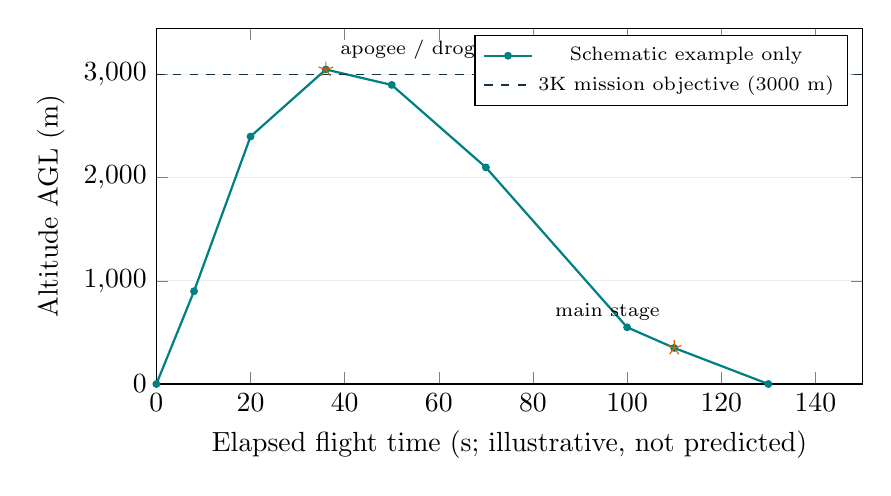
\begin{tikzpicture}
\begin{axis}[width=.87\linewidth,height=6.1cm,xmin=0,xmax=150,ymin=0,ymax=3450,
 xlabel={Elapsed flight time (s; illustrative, not predicted)},ylabel={Altitude AGL (m)},
 ymajorgrids,grid style={gray!15},legend style={font=\scriptsize,at={(.98,.98)},anchor=north east}]
\addplot[thick,teal,mark=*,mark size=1pt] coordinates {(0,0)(8,900)(20,2400)(36,3050)(50,2900)(70,2100)(100,550)(110,350)(130,0)};
\addlegendentry{Schematic example only}
\addplot[Navy,dashed,domain=0:150]{3000};
\addlegendentry{3K mission objective (3000 m)}
\addplot[only marks,mark=star,mark size=2.8pt,color=orange!80!black] coordinates {(36,3050)(110,350)};
\node[font=\scriptsize,anchor=west] at (axis cs:37,3240) {apogee / drogue};
\node[font=\scriptsize,anchor=east] at (axis cs:109,700) {main stage};
\end{axis}\end{tikzpicture}
\caption{\textbf{Illustrative only}: this is \emph{not} the Pioneer-10K trajectory, a flight result or a validated simulation. The actual apogee, peak acceleration, coast time, deployment times and splashdown duration must come from team flight-dynamics analysis. The nominal main-event marker at 350 m is a placeholder within the allowed range.}
\label{fig:missionprofile}
\end{figure}

\subsection*{Outcome criteria to discuss and approve at MDR}
\small
\begin{tabularx}{\linewidth}{@{}L{26mm}Y Y Y@{}}
\toprule\rowcolor{VeryLight}\textbf{Mission area}&\textbf{Full success (team proposed)}&\textbf{Partial success (descriptive)}&\textbf{Failure / noncompliance}\\\midrule
Altitude & Measured apogee at least 3,000 m with valid supporting flight record & Valid flight record but apogee below 3,000 m & No interpretable apogee evidence or flight not achieved\\
Flight-data avionics & All four required outputs available and each reported with time reference; target $\ge90\%$ valid onboard samples & At least two usable outputs but missing data or GPS gaps & Required flight record unrecoverable\\
Recovery & Both stages release as designed; water impact predicted/observed below 12 m/s & One stage fails but rocket is nevertheless recovered; \emph{does not meet planned dual-stage criterion} & No safe descent, lost rocket, or unsafe activation\\
Payload & Both temperature channels achieve declared $\ge90\%$ phase completeness & One channel or reduced completeness, according to Section~\ref{sec:payload} & No interpretable or retrievable payload data\\\bottomrule
\end{tabularx}
\normalsize
\textbf{Interpretation.} The partial-success descriptions are for internal reporting only; they do \emph{not} waive any mandatory competition safety or recovery requirement.


\section{Numbered functional requirements and traceability}
\label{sec:reqmatrix}
% ======================================================================
Each requirement is expressed as a \emph{shall} statement and identifies (i) its RTC source or team-proposed status, (ii) the accountable subsystem and (iii) a planned verification activity. The source clauses are regulatory bases; sampling rates and payload thresholds are preliminary team choices. Structure follows the requirements-matrix example \cite{rtc2027app10}.

\footnotesize
\rowcolors{2}{Pale}{white}
\begin{longtable}{@{}L{12mm}L{71mm}L{33mm}L{34mm}@{}}
\toprule\rowcolor{VeryLight}\textbf{ID}&\textbf{Requirement}&\textbf{Source / status}&\textbf{Owner; verification}\\\midrule\endfirsthead
\toprule\rowcolor{VeryLight}\textbf{ID}&\textbf{Requirement (continued)}&\textbf{Source / status}&\textbf{Owner; verification}\\\midrule\endhead
\bottomrule\endlastfoot
AV-01 & The rocket shall obtain and retain altitude, velocity, acceleration and GPS-trajectory records. & App. 03, Sec. 2.1 \cite{rtc2027app03} & Avionics + GPS; V-02, V-10\\
AV-02 & The avionics shall distinguish launch, ascent, apogee, descent and landing states and record event times. & App. 03, Sec. 4.2; team method & Avionics; V-01\\
AV-03 & The flight logger shall acquire, timestamp and store flight measurements without commanding safety-critical recovery outputs. & Team-derived function supporting AV-01 & Avionics; V-02\\
AV-04 & The system shall preserve flight data despite a radio-link outage or unavailable radio link. & Team design choice supporting AV-01 & Avionics; V-02, V-10\\
AV-05 & The design shall address impact, vibration and sensor error and plan representative ground tests. & App. 03, Sec. 4.1.2 \cite{rtc2027app03} & Avionics; V-01, V-09\\
RC-01 & The recovery system shall provide a drogue release at apogee. & App. 03, Sec. 4.2.2.4 & Recovery; V-01, V-05\\
RC-02 & The recovery system shall provide a main release at a selected lower descent altitude, within the organiser's permitted range. & App. 03, Sec. 4.2.2.4; App. 08 & Recovery; V-01, V-05\\
RC-03 & Recovery activation shall be independent or redundant, including relevant sensors, power and activation functions. & App. 03, Sec. 4.1.3 & Recovery; V-05\\
RC-04 & Recovery release arrangements shall have appropriate redundancy against single failures. & App. 03, Sec. 4.2.2.2 & Recovery; V-05, FMEA\\
RC-05 & A safe/armed method and observable status shall prevent unintended activation during preparation. & App. 03, Sec. 4.6 & Recovery; V-05, V-11\\
RC-06 & The parachute/recovery system shall be designed for water-contact descent speed below 12\,m/s. & App. 03, Sec. 4.2.4 & Recovery + structures; analysis\\
PW-01 & The rocket electrical systems shall operate for more than 1.5 hours in normal operation. & App. 03, Sec. 4.7; App. 08 & Electronics; V-06\\
PW-02 & Batteries and critical wiring shall remain secured under expected launch accelerations and vibration. & App. 03, Secs. 4.4, 4.7 & Electronics + structures; V-06, V-11\\
PW-03 & Independent recovery channels shall not share a power supply whose loss disables both channels. & Team mitigation for RC-03 & Recovery; V-04, V-05\\
PW-04 & Battery selection, fusing, insulation and restraint shall address short circuit, vibration, thermal and transport hazards. & App. 03, Sec. 4.7; team mitigation & Power / Safety; V-06, V-11\\
GPS-01 & The rocket shall carry the organiser-standard 3K GPS beacon. & App. 03, Sec. 5.1 & GPS lead; inspection\\
GPS-02 & The GPS integration shall permit position transmission and retrieval of the position history. & App. 03, Sec. 5.1; App. 08 & GPS lead; V-10\\
GPS-03 & The official beacon location, non-shielded antenna, independent power, mechanical restraint and splash protection shall be identified. & Team integration measure; App. 03, Sec. 5.1 & GPS / Structures; V-14\\
RF-01 & Any team-installed transmitter shall comply with applicable frequency and power rules. & App. 03, Sec. 4.1.4 & GPS/communications; inspection\\
PL-01 & The rocket shall carry an additional mission payload distinct from the standard GPS beacon. & App. 03, Sec. 2.2 & Payload lead; inspection\\
PL-02 & The payload shall follow an allowed operational/retention configuration and not interfere with recovery. & App. 03, Sec. 7.1.1 & Payload + integration; inspection\\
PL-03 & The additional payload shall not contain prohibited stored-energy devices or living vertebrates. & App. 03, Secs. 7.1.2, 7.1.5 & Payload lead; inspection\\
PL-04 & The proposed thermal payload shall obtain two aligned temperature histories and meet declared mission success criteria. & Team mission proposal; \cite{rtc2027app07} & Payload; V-08\\
INT-01 & Electrical interfaces, wiring and mounting shall be identified, supported and strain relieved. & App. 03, Sec. 4.4 & Integration; V-11\\
INT-03 & The avionics bay, media and tracking equipment shall be protected against expected splashdown ingress without compromising barometric sensing. & Team-derived sea-recovery requirement; App. 03, Secs. 4.1, 6.1 & Integration; V-13\\
RC-07 & Recovery controllers shall use an independent flight-state confirmation in addition to barometric altitude before leaving their safe prelaunch state. & Team risk-control derived from RC-03 & Recovery; V-01, V-05\\
INT-02 & The MDR shall include a BOM, schedule, responsibility allocation, risks and verification plan. & App. 01; App. 07 \cite{rtc2027app01,rtc2027app07} & Team lead; review\\
\end{longtable}
\normalsize

\section{Technical issue closure checklist}
%======================================================================
The review of the previous draft raised six technical issues. This revision addresses each one as follows. ``Status'' states honestly what is closed in the document and what still needs team input or hardware evidence.

\small
\rowcolors{2}{Pale}{white}
\begin{longtable}{@{}L{8mm}L{36mm}L{56mm}L{28mm}L{18mm}@{}}
\toprule\rowcolor{VeryLight}\textbf{ID}&\textbf{Technical issue}&\textbf{Closure action in this revision}&\textbf{Status}&\textbf{Where}\\\midrule\endfirsthead
\toprule\rowcolor{VeryLight}\textbf{ID}&\textbf{Issue}&\textbf{Closure action (continued)}&\textbf{Status}&\textbf{Where}\\\midrule\endhead
\bottomrule\endlastfoot
$\square$ A & Three Picos are not automatically independent recovery channels. & Common-cause analysis; diverse barometer and algorithm in channel B; release-interface requirements R1--R4; fault-injection tests. & Analysis done; release mechanism still \status{TBD} (recovery lead). & Sec.~\ref{sec:ccf}\\
$\square$ B & MPU6050 $\pm16$\,g range is not justified against the flight. & Specific-force equation, input list and the ADXL375 $\pm200$\,g as a preliminary baseline high-g channel; saturation flag. & Rule defined; needs Pioneer-10K thrust curve and simulation \status{TBD}. & Sec.~\ref{sec:accel}\\
$\square$ C & Watchdog scratch registers do not protect against power loss. & Corrected claim; reset-cause table; FRAM checkpoint with CRC and double slots; hold-up capacitance; cold-boot rules; revised Fig.~\ref{fig:boot}. & Design defined; to be demonstrated by V-04. & Sec.~\ref{sec:state}\\
$\square$ D & Thermal payload lacks a defined scientific objective. & Research question, hypothesis, uncertainty budget, completeness and retrieval criteria, and what new information results. & Defined; accuracy to be demonstrated by V-08. & Sec.~\ref{sec:payload}\\
$\square$ E & Budget omits recovery controllers, protection, mounting and verification. & Tiered budget separating Shopee-priced parts, allowances and unquoted items, with spares, test costs, contingency and mass estimate. & Provisional; release hardware and GPS beacon unquoted. & Sec.~\ref{sec:budget}\\
$\square$ F & GPS and flight-data outputs lack a defined interface. & Post-flight data pipeline, time-alignment method, merged table and per-output availability criteria. & Defined; beacon file retrieval method to confirm with organiser. & Sec.~\ref{sec:dataflow}\\
\end{longtable}
\normalsize

%======================================================================
\section{Design drivers: how the Pico design meets the 3K criteria}
%======================================================================
The preliminary design uses \textbf{three separate Raspberry Pi Pico boards} (RP2040) \cite{picods,rp2040ds}: one \emph{logger/payload} Pico that never commands recovery, and two \emph{independent recovery} Picos (primary and backup), each with its own barometer, launch-detection IMU and battery. This keeps required flight-data logging and the thermal experiment from sharing a failure path with parachute deployment, while using one familiar, low-cost, well-documented platform for every computer in the rocket.

\small
\rowcolors{2}{Pale}{white}
\begin{longtable}{@{}L{34mm}L{70mm}L{46mm}@{}}
\toprule\rowcolor{VeryLight}\textbf{3K criterion}&\textbf{Design response}&\textbf{Basis / status}\\\midrule\endfirsthead
\toprule\rowcolor{VeryLight}\textbf{3K criterion}&\textbf{Design response (continued)}&\textbf{Basis / status}\\\midrule\endhead
\bottomrule\endlastfoot
Record altitude, velocity, acceleration, GPS trajectory & Logger Pico records BMP280 pressure-altitude and MPU6050 acceleration with timestamps; velocity is derived by filtering/fusion; GPS track is taken from the organiser beacon and merged post-flight (Sec.~\ref{sec:dataflow}). & \cite{rtc2027app03} Sec.~2.1; proposed method\\
Detect launch, apogee, descent & Multi-condition state machine (Figs.~\ref{fig:boot}--\ref{fig:flight}) with lock-outs and time-out back-ups. & \cite{rtc2027app03} Sec.~4.2.2.4; proposed\\
Two-stage recovery: drogue at apogee, main at lower altitude & Two recovery Picos each execute both events; main altitude selected in the 150--450\,m window, below the 500\,m inspection criterion. & \cite{rtc2027app03} 4.2.2.4; \cite{rtc2027app08} Row 8\\
Independent / redundant activation, release redundancy & Primary and backup recovery Picos, separate batteries, independent IMUs, separate barometers, diverse barometer and algorithm in B, outputs held low in hardware (Fig.~\ref{fig:recovery}); common-cause analysis in Sec.~\ref{sec:ccf}. & \cite{rtc2027app03} 4.1.3, 4.2.2.2; mechanism \status{TBD}\\
Safe/armed states, arming confirmation & Arming switch gates power; outputs forced low by pull-downs; launch-inhibit logic; buzzer/LED status code. & \cite{rtc2027app03} 4.6.3--4.6.7\\
Vibration, impact, sensor error & Plausibility gates, filtering, CRC records, strain-relieved connectors, watchdog restart and FRAM state checkpoint (Sec.~\ref{sec:state}). & \cite{rtc2027app03} 4.1.2, 4.4\\
$>1.5$\,h electrical operation & Single Li-ion cell per Pico; load $\approx$56\,mA estimated, 200\,mA design basis (Sec.~\ref{sec:power}). & \cite{rtc2027app03} 4.7.2; \cite{rtc2027app08} Row 6\\
Official GPS tracker & Separate, organiser-standard beacon, own power, no electrical dependence on Pico boards. & \cite{rtc2027app03} 2.2, 5.1\\
Additional payload & Two DS18B20 probes read by the logger Pico: internal avionics-bay vs inner-wall temperature difference with defined research question (Sec.~\ref{sec:payload}); retained in rocket, no radio, no stored-energy device. & \cite{rtc2027app03} 7.1; team proposal\\
No unapproved radio emissions & Plain Pico (not Pico~W): no on-board radio. & \cite{rtc2027app03} 4.1.4; \cite{picods}\\
\end{longtable}
\normalsize

%======================================================================
\section{System architecture}\label{sec:architecture}
%======================================================================
\begin{figure}[ht]
\centering
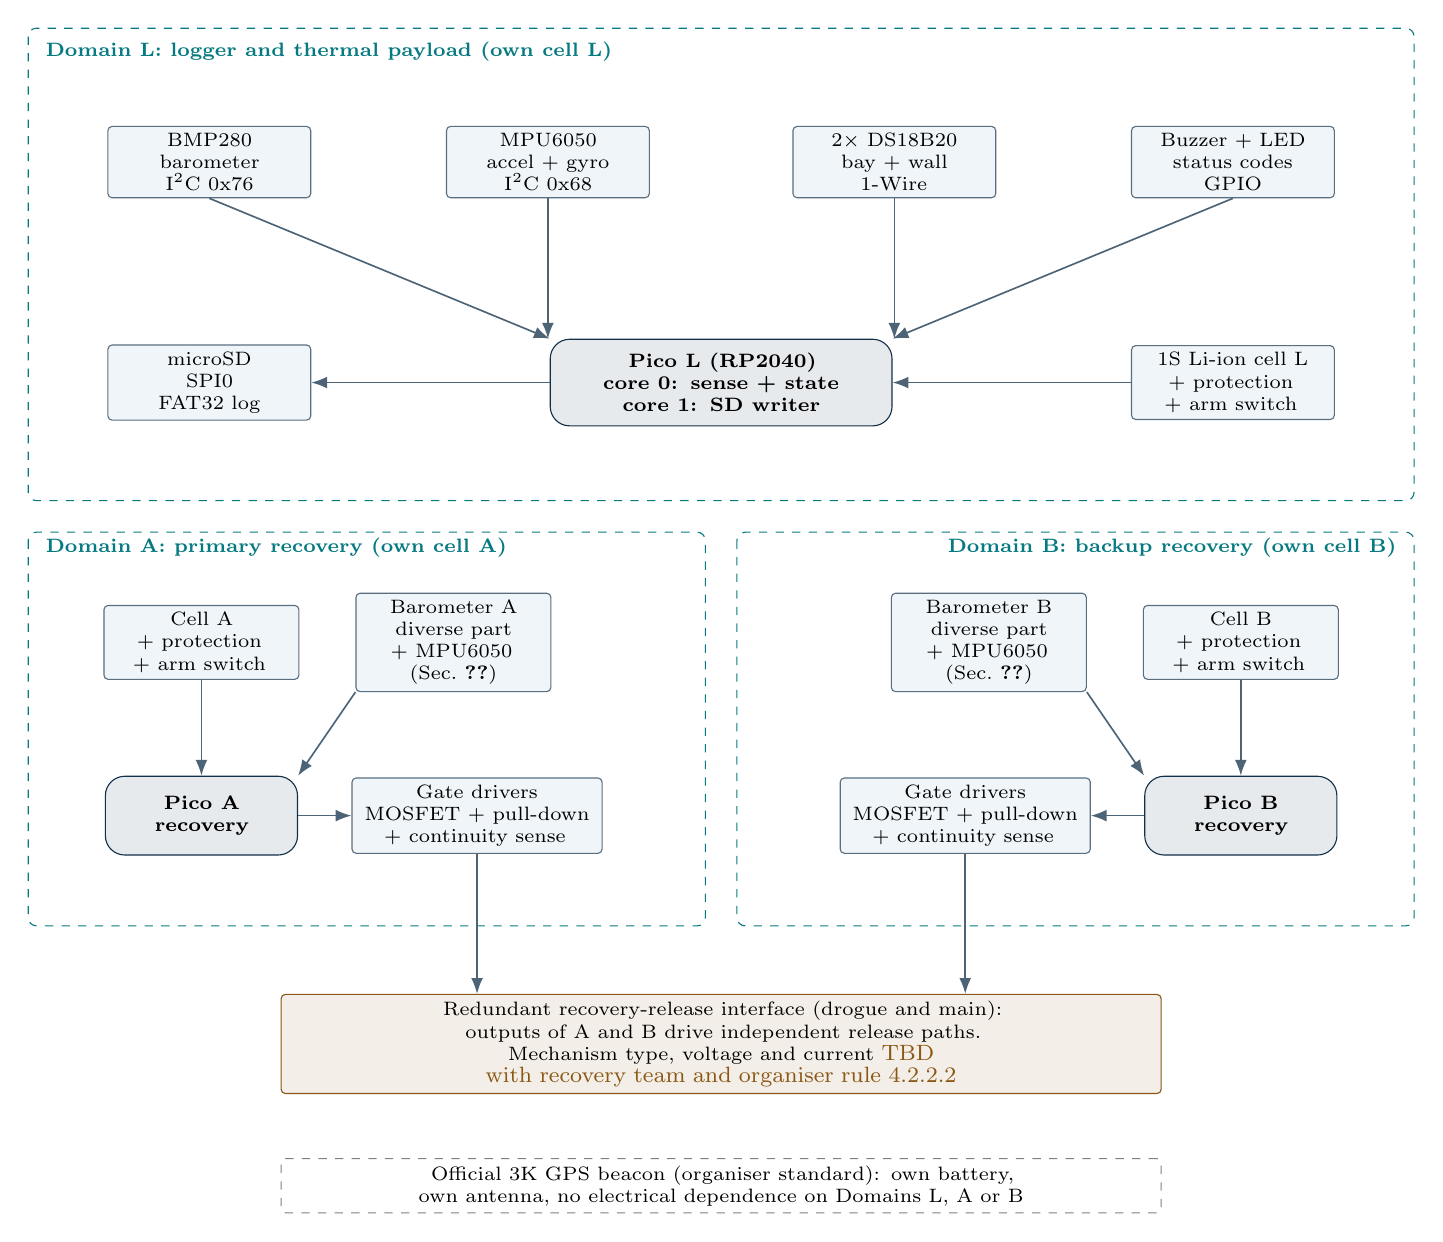
\begin{tikzpicture}[font=\scriptsize]
% ---- logger domain ----
\draw[group] (-8.8,1.0) rectangle (8.8,-5.0);
\node[font=\scriptsize\bfseries,color=Teal,anchor=north west] at (-8.7,0.95) {Domain L: logger and thermal payload (own cell L)};
\node[proc,text width=2.4cm] (bmpL) at (-6.5,-0.7) {BMP280\\barometer\\I$^2$C 0x76};
\node[proc,text width=2.4cm] (mpu)  at (-2.2,-0.7) {MPU6050\\accel + gyro\\I$^2$C 0x68};
\node[proc,text width=2.4cm] (ds)   at (2.2,-0.7)  {2$\times$ DS18B20\\bay + wall\\1-Wire};
\node[proc,text width=2.4cm] (bz)   at (6.5,-0.7)  {Buzzer + LED\\status codes\\GPIO};
\node[term,text width=4.2cm,minimum height=11mm] (picoL) at (0,-3.5) {Pico L (RP2040)\\core 0: sense + state\\core 1: SD writer};
\node[proc,text width=2.4cm] (sd)   at (-6.5,-3.5) {microSD\\SPI0\\FAT32 log};
\node[proc,text width=2.4cm] (batL) at (6.5,-3.5)  {1S Li-ion cell L\\+ protection\\+ arm switch};
\draw[flow] (bmpL.south) -- (picoL.north west);
\draw[flow] (mpu.south) -- (mpu.south |- picoL.north);
\draw[flow] (ds.south) -- (ds.south |- picoL.north);
\draw[flow] (bz.south) -- (picoL.north east);
\draw[flow] (picoL.west) -- (sd.east);
\draw[flow] (batL.west) -- (picoL.east);
% ---- recovery domains ----
\foreach \s/\n/\x/\ba/\bb/\pa/\pb in {-1/A/-6.6/south west/north east/east/west, 1/B/6.6/south east/north west/west/east} {
  \node[proc,text width=2.3cm] (bat\n) at (\x,-6.8) {Cell \n\\+ protection\\+ arm switch};
  \node[proc,text width=2.3cm] (bmp\n) at (\s*3.4,-6.8) {Barometer \n\\diverse part + MPU6050\\(Sec.~\ref{sec:ccf})};
  \node[term,text width=2.3cm,minimum height=10mm] (pico\n) at (\x,-9.0) {Pico \n\\recovery};
  \node[proc,text width=3.0cm] (drv\n) at (\s*3.1,-9.0) {Gate drivers\\MOSFET + pull-down\\+ continuity sense};
  \draw[flow] (bat\n.south) -- (pico\n.north);
  \draw[flow] (bmp\n.\ba) -- (pico\n.\bb);
  \draw[flow] (pico\n.\pa) -- (drv\n.\pb);
}
\draw[group] (-8.8,-5.4) rectangle (-0.2,-10.4);
\draw[group] (0.2,-5.4) rectangle (8.8,-10.4);
\node[font=\scriptsize\bfseries,color=Teal,anchor=north west] at (-8.7,-5.35) {Domain A: primary recovery (own cell A)};
\node[font=\scriptsize\bfseries,color=Teal,anchor=north east] at (8.7,-5.35) {Domain B: backup recovery (own cell B)};
\node[fault,text width=11cm] (rel) at (0,-11.9) {Redundant recovery-release interface (drogue and main): outputs of A and B drive independent release paths.\\Mechanism type, voltage and current \status{TBD with recovery team and organiser rule 4.2.2.2}};
\draw[flow] (drvA.south) -- (drvA.south |- rel.north);
\draw[flow] (drvB.south) -- (drvB.south |- rel.north);
\node[note,text width=11cm,align=center] (gps) at (0,-13.7) {Official 3K GPS beacon (organiser standard): own battery, own antenna, no electrical dependence on Domains L, A or B};
\end{tikzpicture}
\caption{Electronics architecture. Three Pico boards in three power domains; the logger can fail without affecting recovery, and recovery A can fail without affecting recovery B. A FRAM checkpoint memory on each Pico (I$^2$C1, Sec.~\ref{sec:state}) is omitted for clarity. Illustrative; wiring and fault independence remain to be approved.}
\label{fig:arch}
\end{figure}

\textbf{Critical interface rule.} The logger never commands recovery, and nothing on Domain~L (SD card, thermal probes, buzzer) can block a recovery decision. Cross-links between domains are limited to a common ground reference at the release interface if the recovery team requires it; no shared supply \cite{rtc2027app03}.

%======================================================================
\section{Why the Raspberry Pi Pico}
%======================================================================
\small
\rowcolors{2}{Pale}{white}
\begin{longtable}{@{}L{36mm}L{58mm}L{56mm}@{}}
\toprule\rowcolor{VeryLight}\textbf{RP2040 / Pico feature}&\textbf{What it provides}&\textbf{Benefit to the 3K rocket}\\\midrule\endfirsthead
\toprule\rowcolor{VeryLight}\textbf{Feature}&\textbf{What it provides}&\textbf{Benefit (continued)}\\\midrule\endhead
\bottomrule\endlastfoot
Dual Cortex-M0+ cores, up to 133\,MHz & Two independent cores sharing memory \cite{rp2040ds}. & Core~0 senses and decides; core~1 does slow SD writes, so storage latency cannot delay sampling (Fig.~\ref{fig:loop}).\\
264\,kB on-chip SRAM & Fast RAM for buffers \cite{rp2040ds}. & A 5\,s pre-trigger and write-ahead buffer at 44\,B $\times$ 200\,Hz uses about 44\,kB ($\approx$17\% of SRAM).\\
Hardware I$^2$C, SPI, UART, ADC & Two I$^2$C, two SPI, two UART, 12-bit ADC inputs \cite{rp2040ds}. & Covers IMU/baro (I$^2$C), SD (SPI) and battery-voltage monitoring without extra chips.\\
Programmable I/O (PIO) & Eight state machines for custom protocols \cite{rp2040ds}. & Cycle-exact 1-Wire for DS18B20 without blocking the CPU.\\
Watchdog with scratch registers & Reset timer; scratch registers survive a watchdog reset but not a power-on reset \cite{rp2040ds}. & A watchdog reset recovers flight state (Fig.~\ref{fig:boot}); genuine power loss needs separate checkpointing (Sec.~\ref{sec:state}).\\
Wide supply: VSYS 1.8--5.5\,V & On-board buck-boost supply to 3.3\,V \cite{picods}. & A single 3.0--4.2\,V Li-ion cell powers the board directly; the rail holds as the cell discharges.\\
No radio (Pico, not Pico~W) & Plain board without Wi-Fi/Bluetooth \cite{picods}. & Avoids unapproved emissions from the rocket \cite{rtc2027app03}.\\
Open C/C++ SDK, SWD debug, UF2 boot & Free toolchain and bootloader \cite{picosdk}. & Rapid iteration, scripted builds, and the same toolchain on all three boards.\\
Low cost and availability & Retail boards at a few ringgit, drop-in spares. & Three flight computers plus spares fit a student budget; identical hardware simplifies sparing.\\
\end{longtable}
\normalsize

\textbf{Alternatives considered.} An 8-bit AVR such as the ATmega328P has only 2\,kB of SRAM \cite{atmega328ds}, too little for a buffered logger plus filtering. ESP32 devices offer more processing but include Wi-Fi/Bluetooth radios \cite{esp32ds} that must be disabled or justified under the radio rules \cite{rtc2027app03}. The Pico gives enough memory and I/O without a radio at similar cost.

\textbf{Known Pico limits and mitigations.} The Cortex-M0+ has no hardware FPU \cite{rp2040ds}; at 200\,Hz the filter workload is small, but fixed-point or measured float timing will be checked. Flash is external (XIP), so \emph{no flash writes during flight}; recovery events are kept in RAM and dumped after landing \cite{rp2040ds,picosdk}. A Pico dev board is not qualified flight hardware: the independence of A and B, the watchdog, hard-wired pull-downs and testing are what give confidence, not the board itself. The Pico operating range is $-20$ to $+85\,^{\circ}$C \cite{picods}; the bay temperature is measured by the payload.

%======================================================================

\subsection*{Evidence from student-competition rockets}
Published team reports for the 3-km EuRoC \emph{AVES} and \emph{AVES II} projects provide a more relevant architecture comparator than generic vehicle avionics: barometric/IMU sensing, an additional dedicated high-g channel, persistent data storage, telemetry/GNSS and separation of recovery functions \cite{astg2021aves,astg2022aves2}. A 10,000 ft ($3048$ m) IREC 2026 team project also describes separate commercial recovery altimeters, redundant GPS and an independently powered experiment \cite{irec2026sovereignty}. These are \textbf{design precedents} and not proof that the present Pico boards or release design are flight-qualified; the 10,000-ft report is not treated as a completed flight outcome. This rationale motivates the provisional ADXL375 baseline and two separate recovery sensing paths, while the final requirements remain defined by RTC 2027 \cite{rtc2027app03}.


\section{Component-by-component rationale}\label{sec:components}
%======================================================================
\small
\rowcolors{2}{Pale}{white}
\begin{longtable}{@{}L{23mm}L{30mm}L{60mm}L{37mm}@{}}
\toprule\rowcolor{VeryLight}\textbf{Component}&\textbf{Role}&\textbf{Rationale and fit to 3K criteria}&\textbf{Limit / mitigation}\\\midrule\endfirsthead
\toprule\rowcolor{VeryLight}\textbf{Component}&\textbf{Role}&\textbf{Rationale (continued)}&\textbf{Limit / mitigation}\\\midrule\endhead
\bottomrule\endlastfoot
Pico L (logger) & Flight data, state estimate, thermal payload, status. & Satisfies mandatory output list \cite{rtc2027app03}; isolates non-safety functions from recovery. & Not a recovery path. Verified by Fig.~\ref{fig:arch} separation.\\
Pico A / Pico B (recovery) & Barometer + separate IMU for launch confirmation; independent apogee/main control. & Redundant activation and release redundancy \cite{rtc2027app03}; identical code base reduces effort, separate boards and cells remove single points of failure. & Common-cause risk reduced by diversity, not eliminated (Sec.~\ref{sec:ccf}).\\
BMP280 (logger, recovery A) & Pressure/temperature $\rightarrow$ altitude. & Pressure range 300--1100\,hPa covers sea level to well above 3\,km ($\approx$701\,hPa at 3\,km in a standard atmosphere); relative accuracy about $\pm0.12$\,hPa ($\approx\pm1$\,m) \cite{bmp280ds}. Barometric altitude is the standard method for apogee and main-deployment decisions. & Port must see static pressure, vented away from fast airflow; lock-out near burnout/transonic transients; absolute offset removed by pad baseline.\\
MPU6050 (three boards) & Logger motion and independently confirmed launch in both recovery controllers. & 16-bit ADC, programmable $\pm2$ to $\pm16$\,g, 400\,kHz I$^2$C \cite{mpu6050ds,i2cspec}; $\pm16$\,g gives 2048\,LSB/g, ample resolution. & ADXL375 high-g channel is included as preliminary baseline \cite{adxl375ds}; final range is simulation-dependent (Sec.~\ref{sec:accel}); saturation flagged; gyro $\pm2000^{\circ}$/s limits roll-rate capture.\\
DS18B20 $\times$2 & Payload temperatures: avionics bay and inner airframe wall. & Digital 1-Wire, factory calibrated, $-55$ to $+125\,^{\circ}$C, $\pm0.5\,^{\circ}$C (from $-10$ to $+85\,^{\circ}$C), selectable resolution up to 12-bit \cite{ds18b20ds}; many sensors share one wire; 1\,Hz sampling matches the conversion time. & Probe thermal lag; mounting bias; cable strain relief. Powered normally (not parasitic).\\
ADXL375 high-g sensor (logger) & Proposed baseline $\pm200$ g acceleration channel; separate from gyro and low-g IMU. & Direct design precedent for separate high-g sensing is provided by the 3K AVES/AVES II team reports \cite{astg2021aves,astg2022aves2,adxl375ds}. & Module price and flight-range qualification pending.\\
microSD + SPI module & Non-volatile flight log. & SD cards support SPI mode \cite{sdspec} and are handled by the open FatFs library \cite{fatfs}; $\approx$47.52\,MB for 90\,min at 8.8\,kB/s, so even small cards are oversized. & Use a 3.3\,V-native socket and a $\le$32\,GB FAT32 card; log with 512\,B blocks and 1\,s syncs; test under vibration.\\
1S Li-ion cell per board (A, B, L) & Power. & Compact, high energy; 3.0--4.2\,V maps to the Pico VSYS window \cite{picods}; separate cells keep faults isolated (battery safety per \cite{rtc2027app03} 4.7). & Needs protection circuit, fuse, secure holder; verify endurance $>1.5$\,h.\\
MS5611 barometer (recovery B) & Diverse second barometer for channel B. & A different sensor part avoids a shared systematic fault or supply-chain defect in a single part number \cite{ms5611ds,knight1986}. & Different driver and calibration maths; allowance in budget, price unquoted.\\
I$^2$C FRAM (each Pico) & Non-volatile state checkpoint. & Survives power loss, writes in well under 1\,ms and is not subject to the flash-write restriction in flight \cite{fram,rp2040ds}. & Separate bus (I$^2$C1); CRC and double-slot writes (Sec.~\ref{sec:state}).\\
Arming switch + pull-downs & Safe/armed states. & Hard power gate and gate pull-downs keep outputs low regardless of software state, supporting the safe/armed rules \cite{rtc2027app03}. & Accessible from outside the rocket; status code on buzzer/LED.\\
MOSFET gate drivers + continuity sense & Switch the release device, check the circuit. & Logic-level MOSFETs let 3.3\,V GPIO switch higher currents; low-current continuity check proves wiring without activating the release. & Device current and voltage \status{TBD}; flyback/EMI protection required.\\
Buzzer + LED & Self-test and locator. & Immediate pad confirmation of normal operation/arming status \cite{rtc2027app03}; post-landing locator aid. & Not relied on for any flight decision.\\
JST-XH, labelled harness, PCB/proto-board & Interconnect. & Locking connectors, strain relief and labelled wiring support the vibration and wiring rules \cite{rtc2027app03}. & Retention and pull tests.\\
Official GPS beacon & Location after landing. & Required organiser equipment; kept electrically separate \cite{rtc2027app03}. & Installation and cost to confirm.\\
\end{longtable}
\normalsize

%======================================================================
\section{Interfaces and pin allocation (proposed)}
%======================================================================
\small
\rowcolors{2}{Pale}{white}
\begin{tabularx}{\linewidth}{@{}L{22mm}L{40mm}Y@{}}
\toprule\rowcolor{VeryLight}\textbf{Pico}&\textbf{Signal group}&\textbf{Proposed allocation and notes}\\\midrule
Logger (L) & I$^2$C0 (GP4 SDA, GP5 SCL), 400\,kHz & BMP280 and MPU6050 on one bus; 4.7\,k$\Omega$ pull-ups (breakouts may already add them). Keep leads short \cite{i2cspec}.\\
Logger (L) & SPI0 (GP16--GP19) & microSD, 3.3\,V logic; CS pull-up.\\
Logger (L) & 1-Wire via PIO (GP15) & 4.7\,k$\Omega$ pull-up; both DS18B20 on one bus, addressed by ROM code, conversion started for both together.\\
Logger (L) & High-g ADXL375 via second SPI or separately addressed I$^2$C & Preliminary interface must be finalized without a bus-address conflict; reserve pins and verify logger timing.\\
Logger (L) & ADC0 (GP26) & Cell voltage via resistor divider.\\
Logger (L) & GP14 buzzer, GP25 LED & Status codes only.\\
Recovery A/B & I$^2$C0 (GP4/GP5) & Own barometer plus MPU6050 per board (A: BMP280, B: MS5611 \cite{ms5611ds,mpu6050ds}); not shared with L; use separate I$^2$C addresses.\\
Recovery A/B & I$^2$C0 additional MPU6050 & Each board has an independent 6-axis IMU for launch confirmation; two devices share the local I$^2$C bus using different addresses.\\
Recovery A/B & GP10 drogue, GP11 main & To MOSFET gates; external 100\,k$\Omega$ pull-down on each gate in addition to internal pulls.\\
Recovery A/B & GP12/GP13, ADC0 & Continuity sense inputs and cell voltage.\\
All Picos & I$^2$C1 (GP6 SDA, GP7 SCL) & FRAM checkpoint memory on a bus separate from the sensors, so a sensor-bus fault cannot block state saving \cite{fram}.\\
\bottomrule
\end{tabularx}
\normalsize

%======================================================================
\section{Process flowcharts}\label{sec:flowcharts}
%======================================================================
Figures~\ref{fig:boot}--\ref{fig:recovery} describe the software processes. Rounded boxes are start/end, rectangles are processes, diamonds are decisions, and amber boxes are fault or degraded paths. Parameters are in Sec.~\ref{tab:params}.

\begin{figure}[p]
\centering
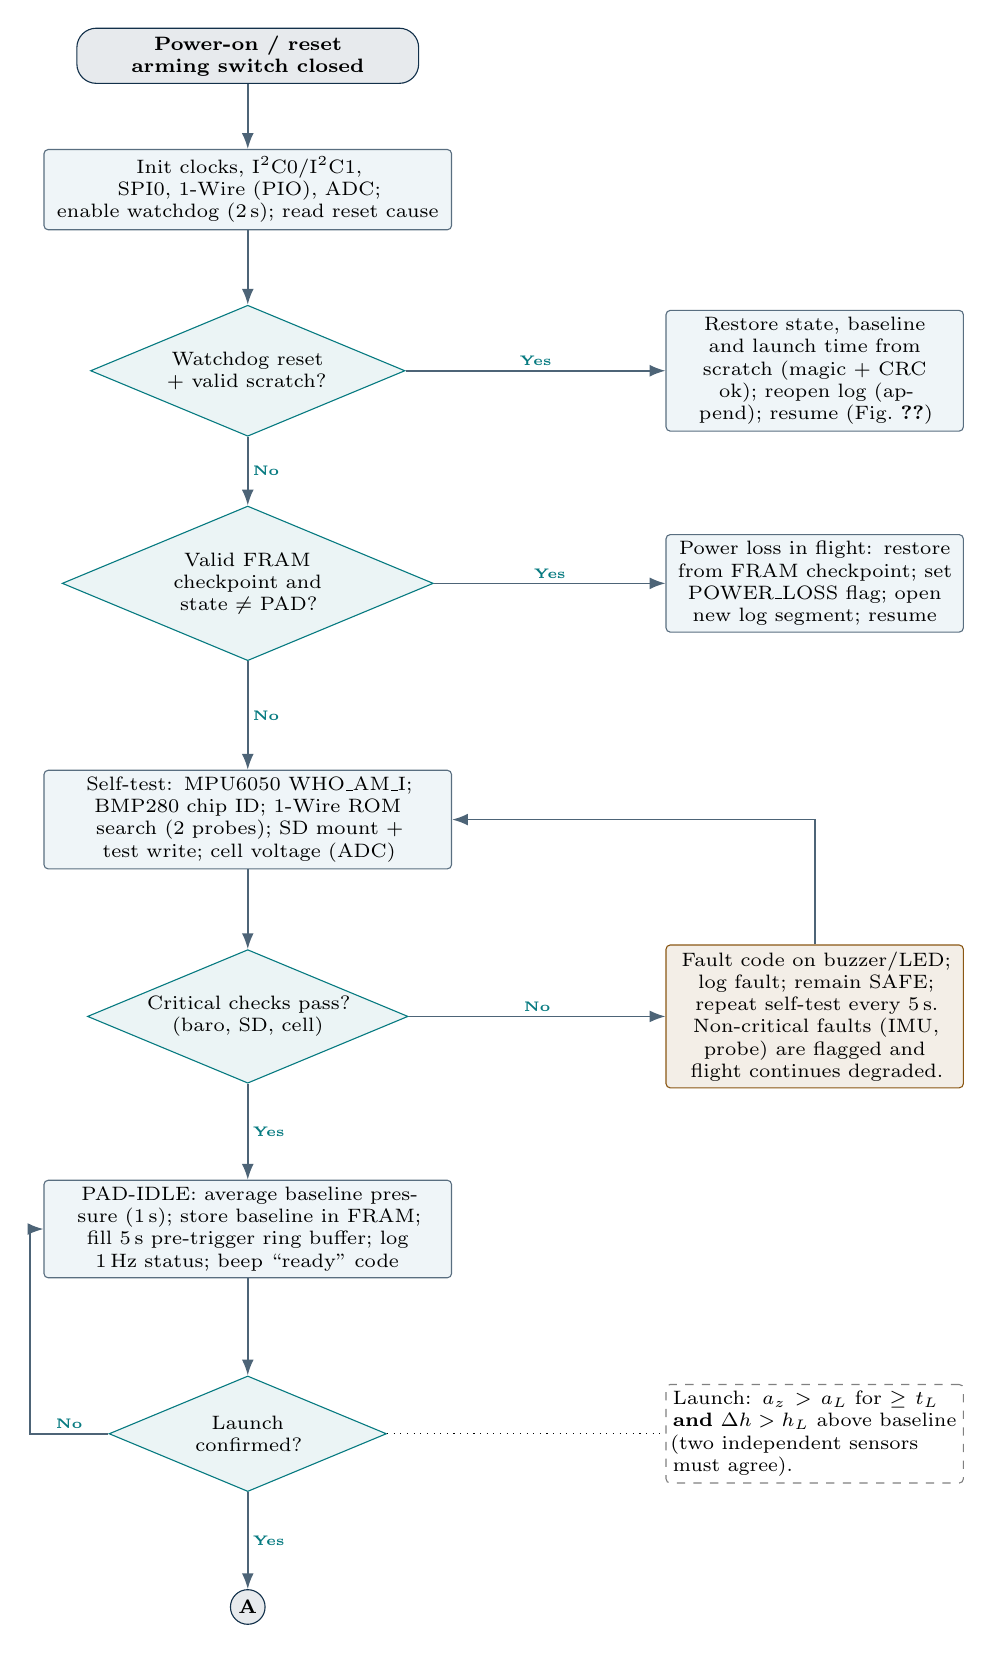
\begin{tikzpicture}
\node[term] (s) at (0,0) {Power-on / reset\\arming switch closed};
\node[proc] (boot) at (0,-1.7) {Init clocks, I$^2$C0/I$^2$C1, SPI0, 1-Wire (PIO), ADC;\\enable watchdog (2\,s); read reset cause};
\node[dec,text width=2.6cm] (d1) at (0,-4.0) {Watchdog reset\\+ valid scratch?};
\node[proc,text width=3.6cm] (rest) at (7.2,-4.0) {Restore state, baseline and launch time from scratch (magic + CRC ok); reopen log (append); resume (Fig.~\ref{fig:flight})};
\node[dec,text width=2.6cm] (d1b) at (0,-6.7) {Valid FRAM\\checkpoint and\\state $\neq$ PAD?};
\node[proc,text width=3.6cm] (rest2) at (7.2,-6.7) {Power loss in flight: restore from FRAM checkpoint; set POWER\_LOSS flag; open new log segment; resume};
\node[proc] (st) at (0,-9.7) {Self-test: MPU6050 WHO\_AM\_I; BMP280 chip ID; 1-Wire ROM search (2 probes); SD mount + test write; cell voltage (ADC)};
\node[dec,text width=2.6cm] (d2) at (0,-12.2) {Critical checks pass?\\(baro, SD, cell)};
\node[fault,text width=3.6cm] (f2) at (7.2,-12.2) {Fault code on buzzer/LED; log fault; remain SAFE; repeat self-test every 5\,s. Non-critical faults (IMU, probe) are flagged and flight continues degraded.};
\node[proc] (idle) at (0,-14.9) {PAD-IDLE: average baseline pressure (1\,s); store baseline in FRAM; fill 5\,s pre-trigger ring buffer; log 1\,Hz status; beep ``ready'' code};
\node[dec] (d3) at (0,-17.5) {Launch\\confirmed?};
\node[note,text width=3.6cm] (n3) at (7.2,-17.5) {Launch: $a_z>a_L$ for $\ge t_L$ \textbf{and} $\Delta h>h_L$ above baseline (two independent sensors must agree).};
\node[conn] (A) at (0,-19.7) {A};
\draw[flow] (s) -- (boot);
\draw[flow] (boot) -- (d1);
\draw[flow] (d1.east) -- node[lab,above]{Yes} (rest.west);
\draw[flow] (d1.south) -- node[lab,right]{No} (d1b.north);
\draw[flow] (d1b.east) -- node[lab,above]{Yes} (rest2.west);
\draw[flow] (d1b.south) -- node[lab,right]{No} (st.north);
\draw[flow] (st) -- (d2);
\draw[flow] (d2.east) -- node[lab,above]{No} (f2.west);
\draw[flow] (f2.north) |- (st.east);
\draw[flow] (d2.south) -- node[lab,right]{Yes} (idle.north);
\draw[flow] (idle) -- (d3);
\draw[flow] (d3.west) -- ++(-1.0,0) node[lab,above,pos=.5]{No} |- (idle.west);
\draw[dotted] (d3.east) -- (n3.west);
\draw[flow] (d3.south) -- node[lab,right]{Yes} (A.north);
\end{tikzpicture}
\caption{Logger Pico start-up with reset-cause discrimination: a watchdog reset restores state from scratch registers; a power loss restores it from the FRAM checkpoint; otherwise a normal self-test and pad-idle run until launch detect.}
\label{fig:boot}
\end{figure}

\begin{figure}[p]
\centering
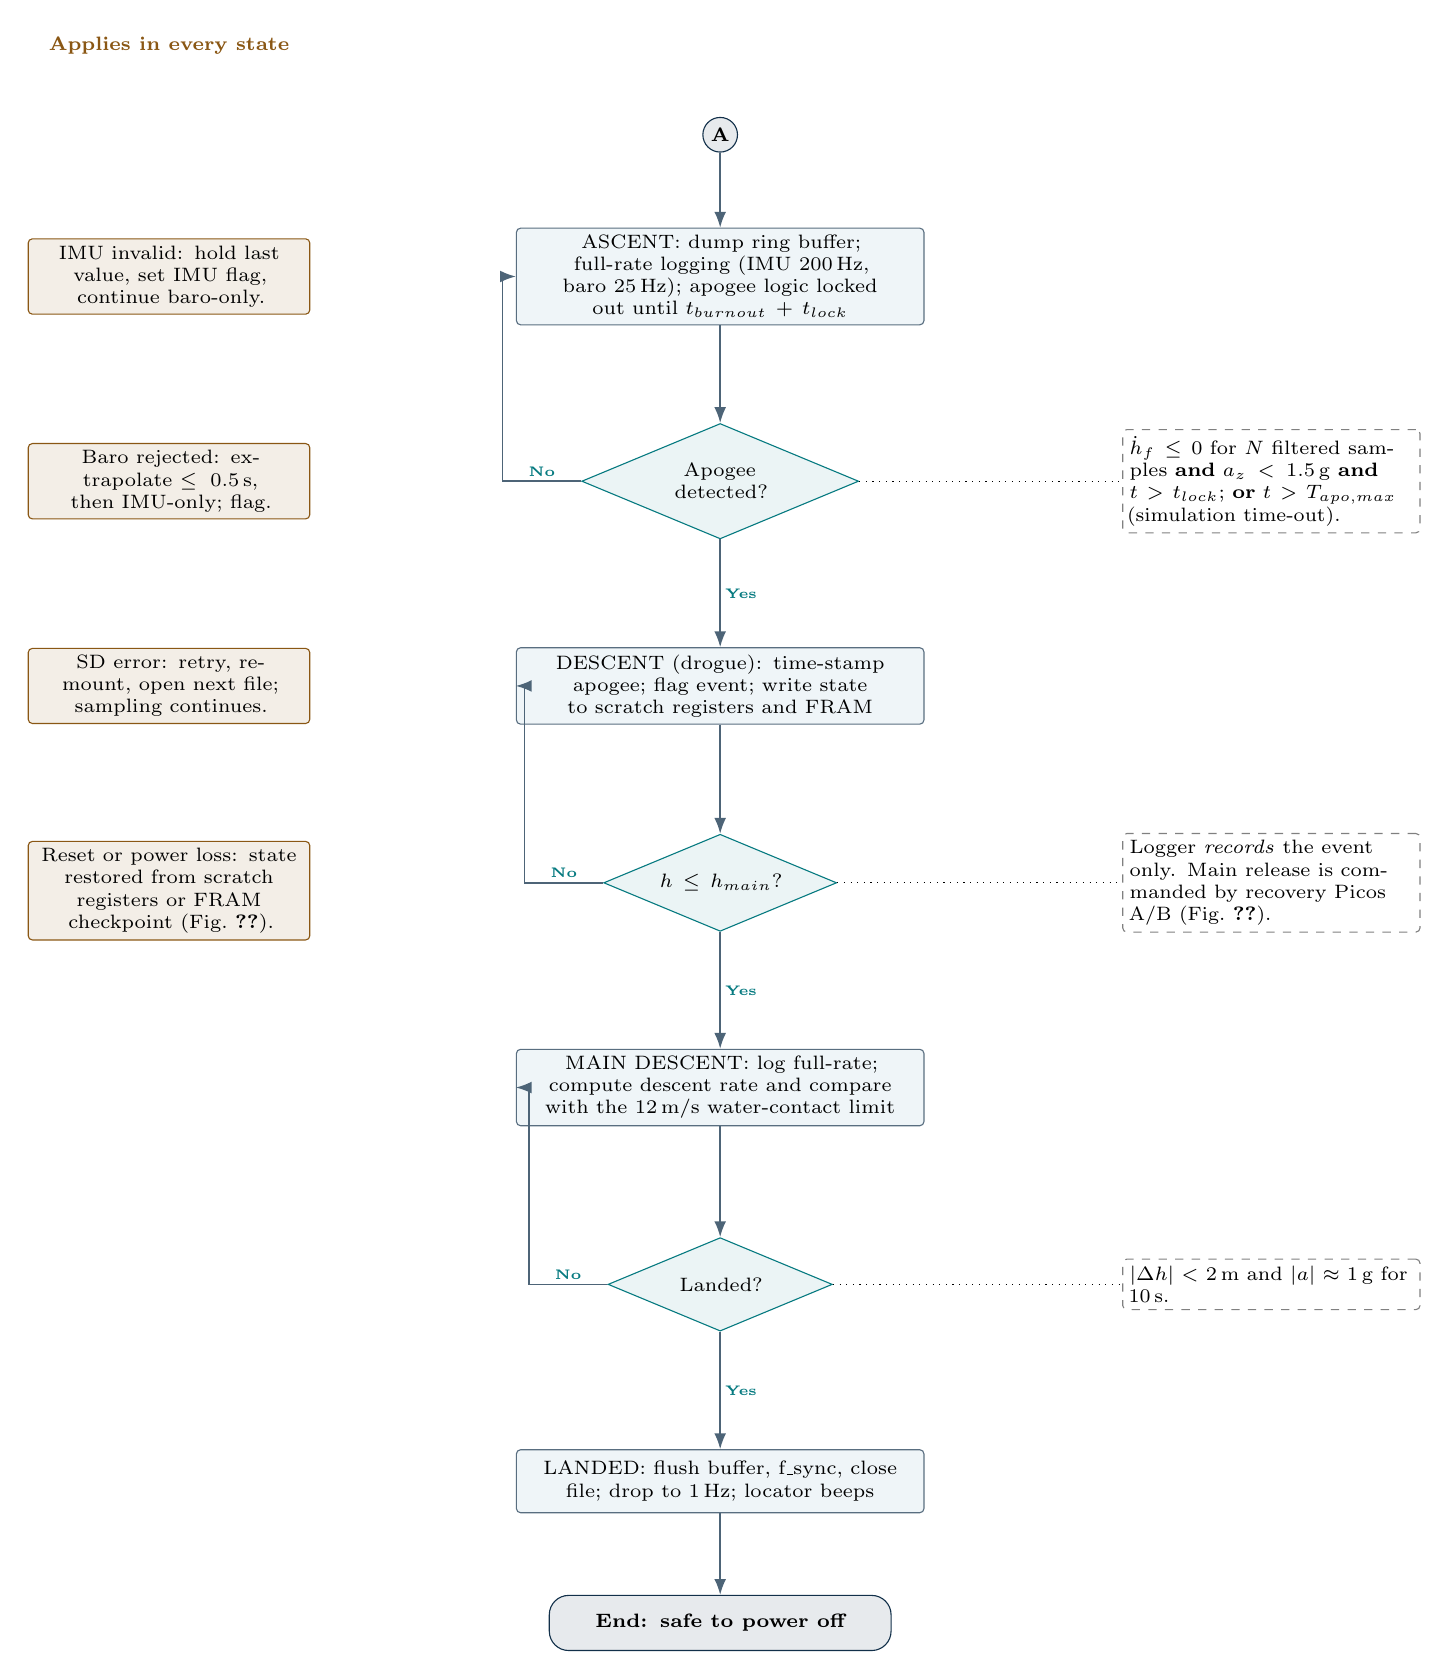
\begin{tikzpicture}
\node[font=\scriptsize\bfseries,color=Amber,anchor=south] at (-7.0,0.9) {Applies in every state};
\node[conn] (A) at (0,0) {A};
\node[proc] (asc) at (0,-1.8) {ASCENT: dump ring buffer; full-rate logging (IMU 200\,Hz, baro 25\,Hz); apogee logic locked out until $t_{burnout}+t_{lock}$};
\node[dec] (d4) at (0,-4.4) {Apogee\\detected?};
\node[note,text width=3.6cm] (n4) at (7.0,-4.4) {$\dot h_f\le0$ for $N$ filtered samples \textbf{and} $a_z<1.5$\,g \textbf{and} $t>t_{lock}$; \textbf{or} $t>T_{apo,max}$ (simulation time-out).};
\node[proc] (drog) at (0,-7.0) {DESCENT (drogue): time-stamp apogee; flag event; write state to scratch registers and FRAM};
\node[dec] (d5) at (0,-9.5) {$h\le h_{main}$?};
\node[note,text width=3.6cm] (n5) at (7.0,-9.5) {Logger \emph{records} the event only. Main release is commanded by recovery Picos A/B (Fig.~\ref{fig:recovery}).};
\node[proc] (main) at (0,-12.1) {MAIN DESCENT: log full-rate; compute descent rate and compare with the 12\,m/s water-contact limit};
\node[dec] (d6) at (0,-14.6) {Landed?};
\node[note,text width=3.6cm] (n6) at (7.0,-14.6) {$|\Delta h|<2$\,m and $|a|\approx1$\,g for 10\,s.};
\node[proc] (land) at (0,-17.1) {LANDED: flush buffer, f\_sync, close file; drop to 1\,Hz; locator beeps};
\node[term] (end) at (0,-18.9) {End: safe to power off};
\node[fault] (a1) at (-7.0,-1.8) {IMU invalid: hold last value, set IMU flag, continue baro-only.};
\node[fault] (a2) at (-7.0,-4.4) {Baro rejected: extrapolate $\le0.5$\,s, then IMU-only; flag.};
\node[fault] (a3) at (-7.0,-7.0) {SD error: retry, remount, open next file; sampling continues.};
\node[fault] (a4) at (-7.0,-9.6) {Reset or power loss: state restored from scratch registers or FRAM checkpoint (Fig.~\ref{fig:boot}).};
\draw[flow] (A) -- (asc);
\draw[flow] (asc) -- (d4);
\draw[flow] (d4.south) -- node[lab,right]{Yes} (drog.north);
\draw[flow] (d4.west) -- ++(-1.0,0) node[lab,above,pos=.5]{No} |- (asc.west);
\draw[dotted] (d4.east) -- (n4.west);
\draw[flow] (drog) -- (d5);
\draw[flow] (d5.south) -- node[lab,right]{Yes} (main.north);
\draw[flow] (d5.west) -- ++(-1.0,0) node[lab,above,pos=.5]{No} |- (drog.west);
\draw[dotted] (d5.east) -- (n5.west);
\draw[flow] (main) -- (d6);
\draw[flow] (d6.south) -- node[lab,right]{Yes} (land.north);
\draw[flow] (d6.west) -- ++(-1.0,0) node[lab,above,pos=.5]{No} |- (main.west);
\draw[dotted] (d6.east) -- (n6.west);
\draw[flow] (land) -- (end);
\end{tikzpicture}
\caption{Logger Pico in-flight state machine. Left column: anomaly handling that applies in all states.}
\label{fig:flight}
\end{figure}

\begin{figure}[p]
\centering
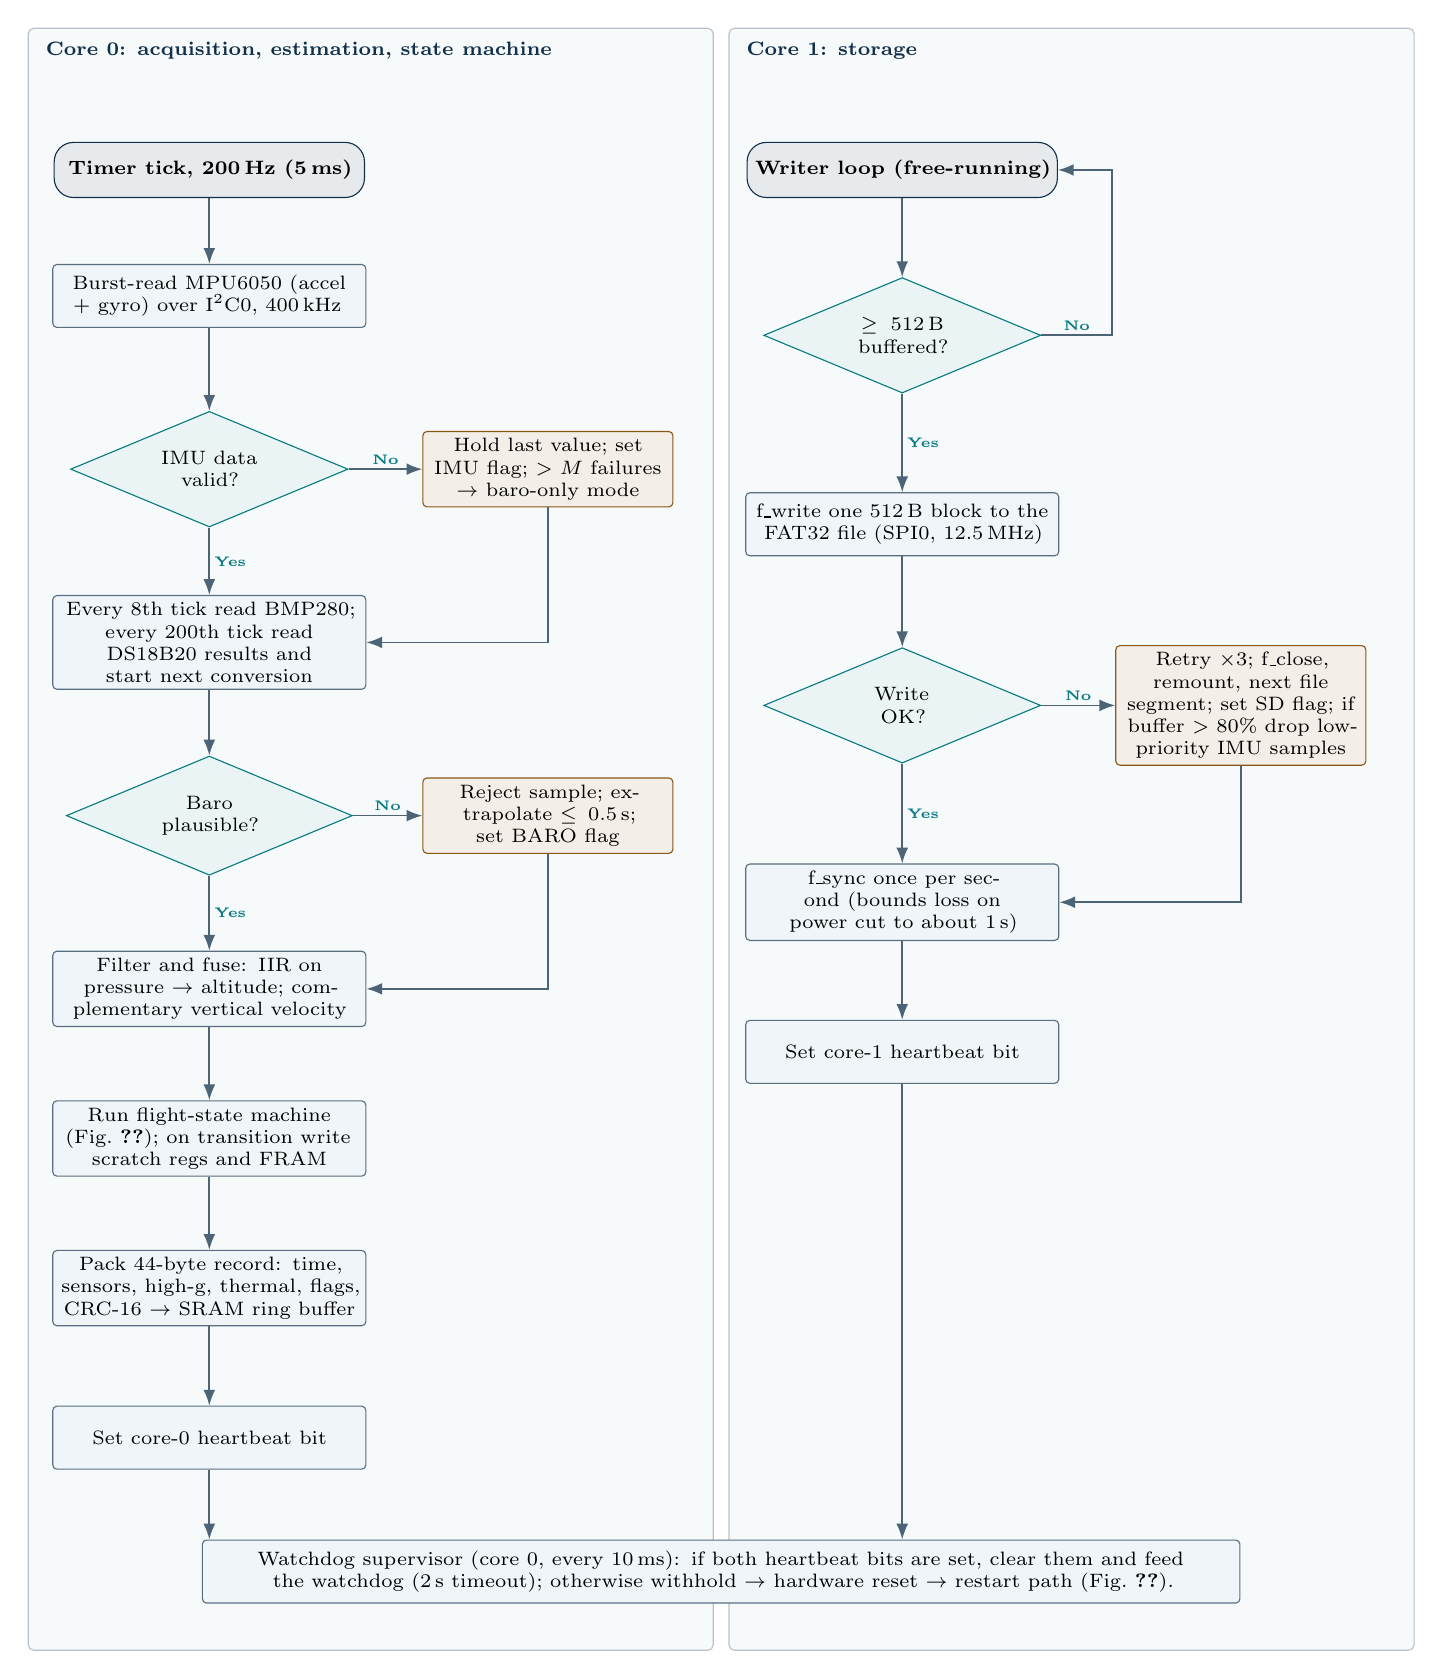
\begin{tikzpicture}
\draw[lane] (-8.8,0.9) rectangle (-0.1,-19.7);
\draw[lane] (0.1,0.9) rectangle (8.8,-19.7);
\node[font=\scriptsize\bfseries,color=Navy,anchor=north west] at (-8.7,0.85) {Core 0: acquisition, estimation, state machine};
\node[font=\scriptsize\bfseries,color=Navy,anchor=north west] at (0.2,0.85) {Core 1: storage};
% core 0
\node[term,text width=3.8cm] (t0) at (-6.5,-0.9) {Timer tick, 200\,Hz (5\,ms)};
\node[proc,text width=3.8cm] (imu) at (-6.5,-2.5) {Burst-read MPU6050 (accel + gyro) over I$^2$C0, 400\,kHz};
\node[dec] (di) at (-6.5,-4.7) {IMU data\\valid?};
\node[fault,text width=3.0cm] (fi) at (-2.2,-4.7) {Hold last value; set IMU flag; $>M$ failures $\rightarrow$ baro-only mode};
\node[proc,text width=3.8cm] (bar) at (-6.5,-6.9) {Every 8th tick read BMP280; every 200th tick read DS18B20 results and start next conversion};
\node[dec] (db) at (-6.5,-9.1) {Baro\\plausible?};
\node[fault,text width=3.0cm] (fb) at (-2.2,-9.1) {Reject sample; extrapolate $\le0.5$\,s; set BARO flag};
\node[proc,text width=3.8cm] (fil) at (-6.5,-11.3) {Filter and fuse: IIR on pressure $\rightarrow$ altitude; complementary vertical velocity};
\node[proc,text width=3.8cm] (fsm) at (-6.5,-13.2) {Run flight-state machine (Fig.~\ref{fig:flight}); on transition write scratch regs and FRAM};
\node[proc,text width=3.8cm] (pk) at (-6.5,-15.1) {Pack 44-byte record: time, sensors, high-g, thermal, flags, CRC-16 $\rightarrow$ SRAM ring buffer};
\node[proc,text width=3.8cm] (hb0) at (-6.5,-17.0) {Set core-0 heartbeat bit};
% core 1
\node[term,text width=3.8cm] (w0) at (2.3,-0.9) {Writer loop (free-running)};
\node[dec] (wd) at (2.3,-3.0) {$\ge512$\,B\\buffered?};
\node[proc,text width=3.8cm] (wr) at (2.3,-5.4) {f\_write one 512\,B block to the FAT32 file (SPI0, 12.5\,MHz)};
\node[dec] (dw) at (2.3,-7.7) {Write\\OK?};
\node[fault,text width=3.0cm] (fw) at (6.6,-7.7) {Retry $\times3$; f\_close, remount, next file segment; set SD flag; if buffer $>80\%$ drop low-priority IMU samples};
\node[proc,text width=3.8cm] (sy) at (2.3,-10.2) {f\_sync once per second (bounds loss on power cut to about 1\,s)};
\node[proc,text width=3.8cm] (hb1) at (2.3,-12.1) {Set core-1 heartbeat bit};
% supervisor
\node[proc,text width=13cm] (sup) at (0,-18.7) {Watchdog supervisor (core 0, every 10\,ms): if both heartbeat bits are set, clear them and feed the watchdog (2\,s timeout); otherwise withhold $\rightarrow$ hardware reset $\rightarrow$ restart path (Fig.~\ref{fig:boot}).};
% flows core 0
\draw[flow] (t0) -- (imu);
\draw[flow] (imu) -- (di);
\draw[flow] (di.south) -- node[lab,right]{Yes} (bar.north);
\draw[flow] (di.east) -- node[lab,above]{No} (fi.west);
\draw[flow] (fi.south) |- (bar.east);
\draw[flow] (bar) -- (db);
\draw[flow] (db.south) -- node[lab,right]{Yes} (fil.north);
\draw[flow] (db.east) -- node[lab,above]{No} (fb.west);
\draw[flow] (fb.south) |- (fil.east);
\draw[flow] (fil) -- (fsm);
\draw[flow] (fsm) -- (pk);
\draw[flow] (pk) -- (hb0);
\draw[flow] (hb0.south) -- (hb0.south |- sup.north);
% flows core 1
\draw[flow] (w0) -- (wd);
\draw[flow] (wd.east) -- ++(0.9,0) node[lab,above,pos=.5]{No} |- (w0.east);
\draw[flow] (wd.south) -- node[lab,right]{Yes} (wr.north);
\draw[flow] (wr) -- (dw);
\draw[flow] (dw.south) -- node[lab,right]{Yes} (sy.north);
\draw[flow] (dw.east) -- node[lab,above]{No} (fw.west);
\draw[flow] (fw.south) |- (sy.east);
\draw[flow] (sy) -- (hb1);
\draw[flow] (hb1.south) -- (hb1.south |- sup.north);
\end{tikzpicture}
\caption{Logger Pico dual-core task flow with fault handling and the cross-core watchdog supervisor. Core~1 absorbs SD latency so core~0 timing is never blocked.}
\label{fig:loop}
\end{figure}

\begin{figure}[p]
\centering
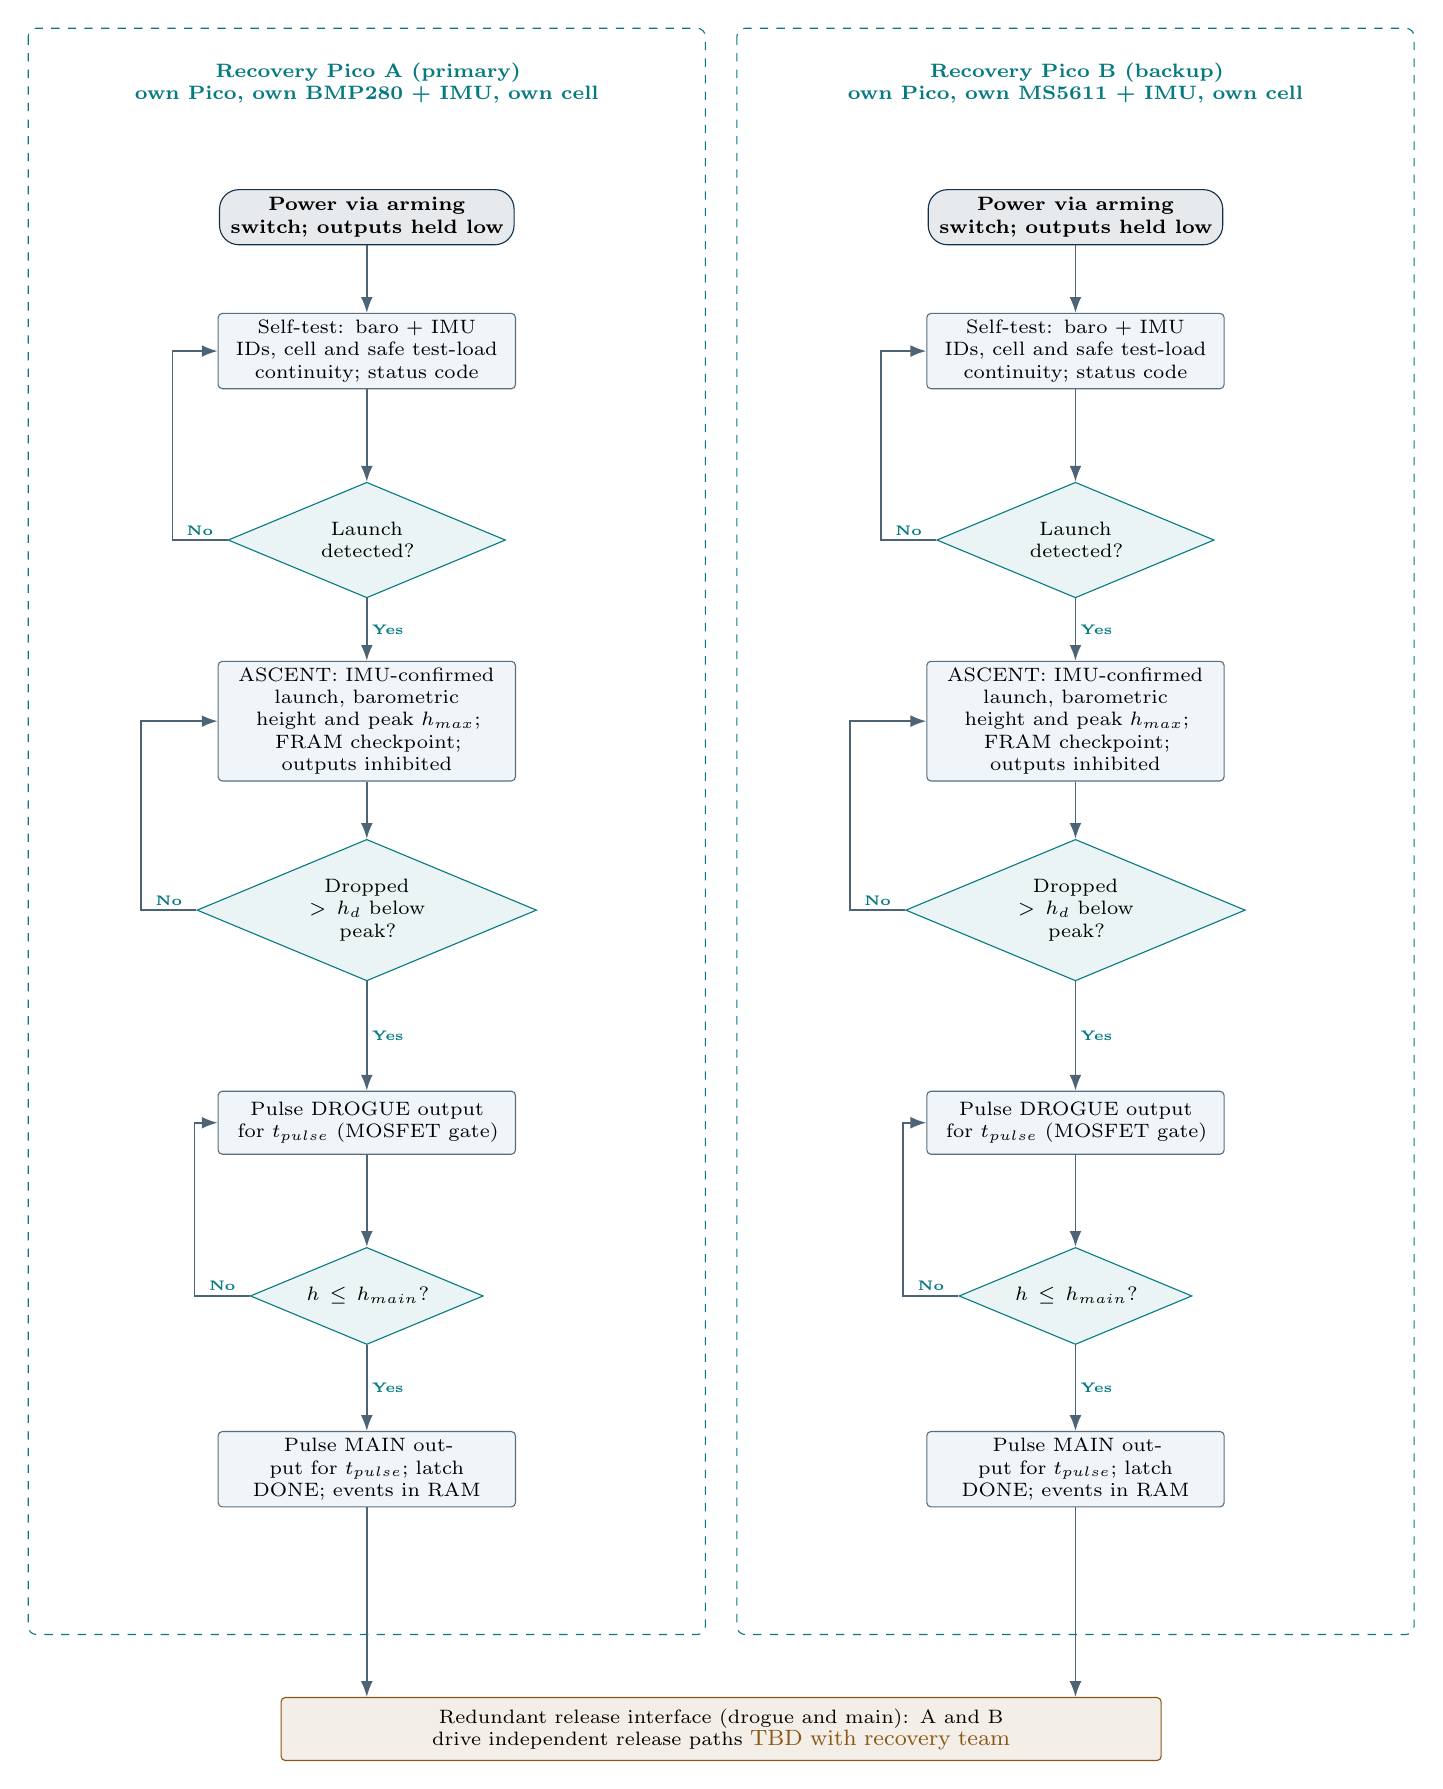
\begin{tikzpicture}
\draw[group] (-8.8,1.9) rectangle (-0.2,-18.5);
\draw[group] (0.2,1.9) rectangle (8.8,-18.5);
\node[font=\scriptsize\bfseries,color=Teal,align=center,text width=8cm] at (-4.5,1.2) {Recovery Pico A (primary)\\own Pico, own BMP280 + IMU, own cell};
\node[font=\scriptsize\bfseries,color=Teal,align=center,text width=8cm] at (4.5,1.2) {Recovery Pico B (backup)\\own Pico, own MS5611 + IMU, own cell};
\foreach \n/\x in {A/-4.5, B/4.5} {
  \node[term,text width=3.6cm] (s0\n) at (\x,-0.5) {Power via arming switch; outputs held low};
  \node[proc,text width=3.6cm] (s1\n) at (\x,-2.2) {Self-test: baro + IMU IDs, cell and safe test-load continuity; status code};
  \node[dec] (d1\n) at (\x,-4.6) {Launch\\detected?};
  \node[proc,text width=3.6cm] (s2\n) at (\x,-6.9) {ASCENT: IMU-confirmed launch, barometric height and peak $h_{max}$; FRAM checkpoint; outputs inhibited};
  \node[dec] (d2\n) at (\x,-9.3) {Dropped\\$>h_d$ below\\peak?};
  \node[proc,text width=3.6cm] (s3\n) at (\x,-12.0) {Pulse DROGUE output for $t_{pulse}$ (MOSFET gate)};
  \node[dec] (d3\n) at (\x,-14.2) {$h\le h_{main}$?};
  \node[proc,text width=3.6cm] (s4\n) at (\x,-16.4) {Pulse MAIN output for $t_{pulse}$; latch DONE; events in RAM};
  \draw[flow] (s0\n) -- (s1\n);
  \draw[flow] (s1\n) -- (d1\n);
  \draw[flow] (d1\n.south) -- node[lab,right]{Yes} (s2\n.north);
  \draw[flow] (d1\n.west) -- ++(-0.7,0) node[lab,above,pos=.5]{No} |- (s1\n.west);
  \draw[flow] (s2\n) -- (d2\n);
  \draw[flow] (d2\n.south) -- node[lab,right]{Yes} (s3\n.north);
  \draw[flow] (d2\n.west) -- ++(-0.7,0) node[lab,above,pos=.5]{No} |- (s2\n.west);
  \draw[flow] (s3\n) -- (d3\n);
  \draw[flow] (d3\n.south) -- node[lab,right]{Yes} (s4\n.north);
  \draw[flow] (d3\n.west) -- ++(-0.7,0) node[lab,above,pos=.5]{No} |- (s3\n.west);
}
\node[fault,text width=11cm] (act) at (0,-19.7) {Redundant release interface (drogue and main): A and B drive independent release paths \status{TBD with recovery team}};
\draw[flow] (s4A.south) -- (s4A.south |- act.north);
\draw[flow] (s4B.south) -- (s4B.south |- act.north);
\end{tikzpicture}
\caption{Independent recovery controllers. Both A and B include IMU-based launch confirmation; B uses a different barometer part and a later apogee trigger, a lower main altitude and an additional time-since-launch back-up compared with A (Secs.~\ref{tab:params} and~\ref{sec:ccf}).}
\label{fig:recovery}
\end{figure}

\subsection{Decision parameters (initial placeholders pending simulation)}
\small
\rowcolors{2}{Pale}{white}
\begin{longtable}{@{}L{22mm}L{58mm}L{66mm}@{}}
\toprule\rowcolor{VeryLight}\textbf{Symbol}&\textbf{Meaning}&\textbf{Starting value / source}\\\midrule\endfirsthead
\toprule\rowcolor{VeryLight}\textbf{Symbol}&\textbf{Meaning}&\textbf{Starting value}\\\midrule\endhead
\bottomrule\endlastfoot
$a_L$, $t_L$ & Launch acceleration threshold and duration (logger and recovery). & e.g.\ 2.5\,g for 50\,ms (10 IMU samples), now including one MPU6050 on each recovery board; set from simulation.\\
$h_L$ & Altitude rise confirming launch. & e.g.\ 10\,m above baseline within 2\,s.\\
$t_{lock}$ & Apogee lock-out after burnout. & Simulation-derived, e.g.\ 1--2\,s, to avoid pressure disturbances near burnout/transonic flight.\\
$N$ & Consecutive filtered samples with $\dot h_f\le0$. & 5 samples at 25\,Hz (0.2\,s).\\
$T_{apo,max}$ & Apogee time-out from launch. & Simulated apogee time $+$ margin.\\
$h_d$ (A / B) & Drop below peak that confirms apogee on recovery boards. & A: small (e.g.\ 3\,m); B: larger (e.g.\ 8\,m) plus delay $\Delta t_B$.\\
$h_{main}$ (A / B) & Main-parachute deployment altitude (AGL). & Within 150--450\,m \cite{rtc2027app03,rtc2027app08}; B set about 30\,m lower than A.\\
$t_{pulse}$ & Output pulse duration. & From release-device specification \status{TBD}.\\
$v_{max}$ & Baro plausibility limit on $|dh/dt|$. & Simulated peak speed $\times$ margin \status{TBD}.\\
\end{longtable}
\normalsize
\label{tab:params}

%======================================================================
\section{Recovery independence and common-cause failure analysis}
\label{sec:ccf}
%======================================================================
Separate boards, cells and barometers remove many single-point failures, but they do not by themselves make two channels independent: a shared design defect, a shared pressure environment or a shared release element can defeat both. Software ``independence'' in particular should not be assumed, because independently written programs have been shown to fail on the same inputs more often than independence would predict \cite{knight1986}. The design therefore combines \emph{diversity}, a \emph{qualitative common-cause analysis} and \emph{fault-injection tests}. Redundancy reduces common-cause risk; it does not eliminate it.

\small
\rowcolors{2}{Pale}{white}
\begin{longtable}{@{}L{25mm}L{38mm}L{52mm}L{35mm}@{}}
\toprule\rowcolor{VeryLight}\textbf{Shared element}&\textbf{Common-cause failure}&\textbf{Countermeasure}&\textbf{Residual / evidence}\\\midrule\endfirsthead
\toprule\rowcolor{VeryLight}\textbf{Shared element}&\textbf{Common-cause failure}&\textbf{Countermeasure (continued)}&\textbf{Residual / evidence}\\\midrule\endhead
\bottomrule\endlastfoot
Software logic & Same defect or same wrong threshold in A and B. & Separate firmware builds written and reviewed by different members; B adds a time-since-launch back-up and different $h_d$ and $h_{main}$ (Sec.~\ref{tab:params}). & Diversity helps but is imperfect \cite{knight1986}; V-01 replay, V-05.\\
Barometer part & Systematic offset, noise or supply defect in one part number. & A uses BMP280 \cite{bmp280ds}, B uses MS5611 \cite{ms5611ds}; different drivers and calibration code. & Both read the same atmosphere; see port row.\\
Static pressure port & Blocked or disturbed port, bay leak, transonic or burnout pressure transient. & Separate ports at different circumferential positions; lock-out $t_{lock}$; B back-up timer; vented-bay pressure test. & Residual common pressure field; V-09.\\
Power & Single cell or connector failure. & Separate cells, switches and harnesses; no shared supply; common ground only at the release interface if required. & V-06, V-08.\\
Release mechanism & One mechanical or electrical element defeats both channels. & Requirements R1--R4 below; independent initiators per channel. & Mechanism \status{TBD}; V-05.\\
Environment & Vibration, shock, temperature or EMI affects both boards. & Separate mounting, distance between boards, strain-relieved wiring, measured bay temperature. & Vibration and thermal tests.\\
Human error & Wrong thresholds, wiring or arming sequence on both boards. & Configuration checksum shown on the status code at arming, labelled harnesses, two-person checklist. & Inspection at integration.\\
\end{longtable}
\normalsize

\textbf{Release-interface requirements (proposed).}
\begin{enumerate}[label=R\arabic*.]
\item Each channel (A and B) shall be able to release both drogue and main without the other channel's power or logic.
\item No single mechanical or electrical element shall prevent both channels from releasing, consistent with the release-redundancy rule \cite{rtc2027app03} (Sec.~4.2.2.2); if a mechanism is shared, the shared element and its redundant initiators shall be documented.
\item All outputs are de-energised by default, and each channel's supply passes through its own arming switch.
\item Compliance is shown by fault injection: A disabled, B disabled, and both enabled, each with safe test loads (V-05).
\end{enumerate}
\textbf{Flight-state sensing clarification.} Each recovery Pico now carries its own MPU6050 and barometer. A tentative launch gate combines sustained acceleration and a separate altitude-rise check; the exact thresholds, persistence and sensor-fault handling require simulation and tests. A barometric fault can still compromise apogee detection, so a \emph{simulation-derived post-launch backup timer} for channel B is proposed as an additional safety analysis item, not an approved flight setting. A board unable to verify its state remains a documented residual risk; this report does not claim that sensor duplication alone ensures deployment.

Candidate arrangements, to be selected with the recovery lead: (i) a common release mechanism with two independent initiators, one per channel; or (ii) two separate mechanisms, subject to the rules. The choice is needed before the MDR text is frozen so that this interface is no longer \status{TBD}.

%======================================================================

% ======================================================================
\section{Preliminary recovery release interface and safe integration}
\label{sec:release}
% ======================================================================
\textbf{Provisional MDR baseline (not a qualified release design).} The recovery team will evaluate a \emph{non-pyrotechnic, spring-assisted retained-door / latch concept} with two electrically independent initiation paths for each parachute stage. The primary recovery controller A and backup controller B will each have their own protected supply and individually isolated switching interface. Either channel must be capable of initiating the relevant stage without the other controller. Spring/servo, latch geometry, actuation current, release force, mechanical redundancy and compatibility with organiser rules are \status{PENDING RECOVERY-LEAD APPROVAL} \cite{rtc2027app03,bakirci2022recovery}.

\small
\rowcolors{2}{Pale}{white}
\begin{tabularx}{\linewidth}{@{}L{34mm}Y L{44mm}@{}}
\toprule\rowcolor{VeryLight}\textbf{Interface}&\textbf{MDR-level design requirement}&\textbf{Evidence / owner}\\\midrule
Electrical initiators & A and B shall have independently powered means to request drogue and main release; no shared active component may block both. & Recovery lead; schematic at PDR\\
Safe/armed control & Both circuits default to a non-energised safe state; arming and status confirmation remain accessible when the rocket is assembled. & Recovery lead; bench demonstration\\
Mechanical interfaces & Release modules, chute bays and harness mounts shall be dimensioned and checked for opening under load and vibration. & Recovery + structures; CAD and tests\\
Electrical envelope & Release-device voltage, stall/peak current, energy requirement and protective devices shall be calculated once the hardware is selected. & Electronics; driver and battery design\\
Fault injection & Verify with safe inert loads: A disabled, B disabled, bus faults, reset and short supply interruptions. & Recovery; V-04 and V-05\\
\bottomrule
\end{tabularx}
\normalsize

This baseline closes the MDR need to \emph{explain a candidate interface}, not the later requirement to qualify it. The actual release mechanism must be agreed with the recovery team and approved by the organiser before construction; the present report does not claim that a consumer servo or untested spring arrangement is flight-qualified.

\section{Accelerometer range decision}
\label{sec:accel}
%======================================================================
The MPU6050 offers programmable ranges up to $\pm16$\,g \cite{mpu6050ds}. Whether that is enough depends on the rocket. An accelerometer measures specific force along its axis, which in g is
\begin{equation}
a_{sf}(t)=\frac{T(t)-D(t)}{m(t)\,g_0},
\end{equation}
where $T$ is thrust, $D$ drag, $m$ the (decreasing) mass and $g_0=9.81$\,m/s$^2$. Parachute-deployment shock must also be included. The inputs are listed below; the Pioneer-10K thrust curve and the team flight simulation were not part of the material used for this revision, so the numerical result is \status{TBD}.

\small
\rowcolors{2}{Pale}{white}
\begin{tabularx}{\linewidth}{@{}L{42mm}Y L{34mm}@{}}
\toprule\rowcolor{VeryLight}\textbf{Input}&\textbf{Use}&\textbf{Status}\\\midrule
Pioneer-10K thrust curve $T(t)$ and burn time & Peak thrust and thrust tolerance. & \status{TBD}\\
Mass history $m(t)$, burnout mass & Peak $a_{sf}$ occurs near low mass. & \status{TBD}\\
Drag $D(t)$ from flight simulation & Net specific force, transonic region. & \status{TBD}\\
Drogue and main deployment shock & Short-duration peaks that may exceed boost peak. & \status{TBD} (analysis, later test)\\
Margin factor $k$ & Covers thrust variation and simulation error. & $k=1.25$ (team assumption)\\
\bottomrule
\end{tabularx}
\normalsize

\textbf{Decision rule.} Let $a_{pk}$ be the largest predicted $|a_{sf}|$ over the whole flight including deployment shock. The proposed logger \emph{includes} a $\pm200$\,g ADXL375 channel in its baseline and retains the MPU6050 for lower-g motion and gyro data. The range adequacy for both sensors must still be established from the simulation and shock envelope. Price is a provisional allowance, not an independently verified Shopee quote. In every case the logger sets a saturation flag when a raw sample reaches full scale, and launch detection still works because it is a threshold crossing well below full scale. Barometric velocity and altitude remain available even if the acceleration record clips. Verification is analysis V-07.

%======================================================================
\section{State preservation across resets and power interruption}
\label{sec:state}
%======================================================================
A watchdog is not a power-loss protection. The RP2040 watchdog scratch registers persist through a \emph{watchdog reset}, but they must not be assumed to survive a power-on reset, a loss of supply or a brown-out \cite{rp2040ds}; the exact behaviour for an external reset (RUN pin) should be re-read in the datasheet before the design is frozen. The design therefore treats the reset causes separately.

\small
\rowcolors{2}{Pale}{white}
\begin{longtable}{@{}L{35mm}L{36mm}L{70mm}@{}}
\toprule\rowcolor{VeryLight}\textbf{Event}&\textbf{Scratch registers}&\textbf{State-preservation strategy}\\\midrule\endfirsthead
\toprule\rowcolor{VeryLight}\textbf{Event}&\textbf{Scratch registers}&\textbf{Strategy (continued)}\\\midrule\endhead
\bottomrule\endlastfoot
Software lock-up caught by watchdog & Retained \cite{rp2040ds} & Restore from scratch registers only if magic number and CRC are valid; otherwise fall through to the FRAM checkpoint.\\
Brief supply dip or brown-out & Not relied on & Hold-up capacitance rides through short dips; if the Pico still restarts, restore from the FRAM checkpoint.\\
Complete power interruption (cell or connector) & Lost & Cold boot, restore from the FRAM checkpoint (if valid), set POWER\_LOSS flag, open a new log segment.\\
External reset line pulse & Do not assume & Same as complete power interruption.\\
No valid checkpoint & Lost & Logger: restart as PAD or fallback per rule below. Recovery boards: see cold-boot rules.\\
\end{longtable}
\normalsize

\textbf{Checkpoint record.} Each checkpoint is a \textbf{32-byte packed record} in I$^2$C FRAM \cite{fram}: 4-byte magic, 1-byte version, 1-byte flight state, 2-byte general flags, 4-byte sequence number, 4-byte launch time, 4-byte baseline pressure, 4-byte peak altitude, 2-byte deployment event flags, 4-byte reserved data, and a 2-byte CRC-16 (total $4+1+1+2+4+4+4+4+2+4+2=32$ bytes). Two alternating slots permit recovery from interrupted writes. At 400 kHz, a 32-byte write with three bytes of address/control overhead takes at least $(32+3)\times9/400000\approx0.79$ ms before additional bus/firmware overhead; actual time must be measured \cite{i2cspec}. Checkpoint at state transitions and periodically, with the proposed 250 ms period to be validated. No flash is written in flight \cite{rp2040ds}.

\textbf{Hold-up.} A bulk capacitor across the board supply keeps the rail up during a brief interruption: $C\approx I\,\Delta t/\Delta V$. For example, 60\,mA for 20\,ms with 0.5\,V allowable droop needs about 2.4\,mF. The value is to be sized and tested, not assumed.

\textbf{Cold-boot rules for recovery boards (proposed).}
\begin{itemize}
\item Outputs are held low from the first instant of boot by the hardware pull-downs; software never energises an output during start-up.
\item With a valid checkpoint in an in-flight state, restore state and continue the normal logic; outputs stay inhibited until their trigger conditions are satisfied again.
\item With no valid checkpoint, the board cannot know the pad baseline. A fallback rule is needed from the recovery lead; one candidate is to inhibit the drogue unless a sustained descent is measured, and to use the main-altitude trigger with the nominal site pressure. The other channel provides primary protection \status{rule TBD}.
\end{itemize}
Verification is by supply-interruption tests in every state (V-04).

%======================================================================
\section{Additional payload: thermal-environment mission definition}
\label{sec:payload}
%======================================================================
\textbf{Research question.} How does the temperature difference between the avionics bay and the inside surface of the airframe wall evolve through the pad, ascent, coast and descent phases of the 3K flight?

\textbf{Hypothesis and null result.} The difference $\Delta T(t)=T_{wall}(t)-T_{bay}(t)$ changes between phases by more than the measurement uncertainty. A flight in which no change larger than the uncertainty is observed is also a valid, reportable result.

\textbf{New information.} The data show whether the avionics bay stays well inside the Pico operating range of $-20$ to $+85\,^{\circ}$C \cite{picods}, how large the bay-to-wall gradient is during flight, and how quickly the bay follows the structure. This supports placement and thermal margin decisions for later flights. The payload stays inside the rocket, is read by the logger and has no radio or stored-energy device; the in-body configuration with avionics communication throughout flight is the one proposed \cite{rtc2027app03} (Sec.~7.1.1).

\small
\rowcolors{2}{Pale}{white}
\begin{longtable}{@{}L{36mm}L{110mm}@{}}
\toprule\rowcolor{VeryLight}\textbf{Item}&\textbf{Definition (team proposal)}\\\midrule\endfirsthead
\toprule\rowcolor{VeryLight}\textbf{Item}&\textbf{Definition (continued)}\\\midrule\endhead
\bottomrule\endlastfoot
Measurements & $T_{bay}$ and $T_{wall}$ from two DS18B20 probes \cite{ds18b20ds}, 1\,Hz each, 12-bit, with sensor ID, timestamp, flight state and validity flag.\\
Phases & Pad (baseline), ascent (launch to burnout), coast (burnout to apogee), descent (apogee to landing), all from the logger state record (Fig.~\ref{fig:flight}).\\
Recording window & From arming through landing plus a post-landing period; expected duration from flight simulation, well inside the $>1.5$\,h battery endurance.\\
Accuracy & Each probe is specified at $\pm0.5\,^{\circ}$C from $-10$ to $+85\,^{\circ}$C \cite{ds18b20ds}; uncalibrated, $\Delta T$ is within $\pm1.0\,^{\circ}$C worst case ($\approx0.7\,^{\circ}$C root-sum-square). After both probes are offset-calibrated in a common stable bath, the target is a $\Delta T$ uncertainty of $\le0.3\,^{\circ}$C, to be demonstrated in V-08.\\
Response time & Probe step response measured on the bench so that lag between bay and wall probes is not mistaken for a physical gradient.\\
\textbf{Success} & Both channels valid for $\ge90\%$ of expected samples in each of the ascent, coast and descent phases; records retrieved with CRC pass $\ge99\%$; phase-mean $\Delta T$ and uncertainty reported.\\
\textbf{Partial success} & One channel valid $\ge90\%$, or both channels valid for 50--89\% of expected samples in at least two phases.\\
\textbf{Failure} & Fewer than 50\% valid samples in the flight window, no retrieved file, or data that cannot be aligned to flight events.\\
Retrieval evidence & Recovered SD card, intact raw file with hash, processed $\Delta T(t)$ plot per phase, completeness table and quality log (Sec.~\ref{sec:dataflow}).\\
\end{longtable}
\normalsize

%======================================================================
\section{Robustness and fault handling}
%======================================================================
\small
\rowcolors{2}{Pale}{white}
\begin{longtable}{@{}L{34mm}L{50mm}L{62mm}@{}}
\toprule\rowcolor{VeryLight}\textbf{Failure mode}&\textbf{Consequence}&\textbf{Mitigation (see flowcharts)}\\\midrule\endfirsthead
\toprule\rowcolor{VeryLight}\textbf{Failure mode}&\textbf{Consequence}&\textbf{Mitigation}\\\midrule\endhead
\bottomrule\endlastfoot
Logger lock-up & Gaps in data or payload record. & Watchdog restart with scratch-register restore; 1\,s sync.\\
Power interruption in flight & Cold boot, loss of state and baseline. & FRAM checkpoint, hold-up capacitance, new log segment with POWER\_LOSS flag (Sec.~\ref{sec:state}).\\
Barometer noise, spike or port blockage & False apogee or main trigger. & Plausibility gate, IIR filter, multi-condition apogee, lock-out, time-out.\\
IMU saturation & Bad launch/burnout and acceleration data. & Range decision gate (Sec.~\ref{sec:accel}), saturation flag, baro cross-check.\\
SD write stall or removal & Missing records. & Core-1 offload, 44\,kB buffer, retry/remount, next-file segment.\\
Recovery A failure & No or late deployment. & Backup B: separate board, diverse sensor, cell, later trigger and time back-up.\\
Common-cause failure of A and B & No deployment on both channels. & Diversity, release requirements R1--R4, fault-injection tests (Sec.~\ref{sec:ccf}).\\
Beacon track missing or misaligned & Incomplete flight-data package. & Redundant altitude sources, time-alignment check, quality flags (Sec.~\ref{sec:dataflow}).\\
Premature output from noise/boot & Unsafe activation. & Outputs held low by pull-downs, arming switch, launch-inhibit logic.\\
Thermal probe detaches & Invalid payload data; loose object. & Mechanical retention, strain relief, flag in record.\\
Connector loosening & Intermittent power/data. & Locking connectors, strain relief, vibration test \cite{rtc2027app03}.\\
\end{longtable}
\normalsize
The full FMEA follows the organiser template \cite{rtc2027app12}; classical FMECA practice is described in \cite{mil1629a}.

%======================================================================
\section{Power and data budgets}
\label{sec:power}
%======================================================================
\textbf{Load estimate (logger).} Values are datasheet-typical or assumed, and must be replaced by measurements.

\small
\rowcolors{2}{Pale}{white}
\begin{tabularx}{\linewidth}{@{}L{48mm}r Y@{}}
\toprule\rowcolor{VeryLight}\textbf{Item}&\textbf{mA}&\textbf{Basis}\\\midrule
Pico L at 125\,MHz, both cores & 30 & Assumed; measure \cite{rp2040ds}\\
MPU6050 (gyro + accel) & 3.9 & Datasheet typical \cite{mpu6050ds}\\
BMP280 & $<0.1$ & Datasheet \cite{bmp280ds}\\
2$\times$ DS18B20 active & 2 & About 1\,mA each \cite{ds18b20ds}\\
microSD module average & 20 & Assumed; write peaks higher\\
\midrule
\textbf{Total estimate} & \textbf{$\approx$56} & Design basis kept at \textbf{200\,mA}\\
\bottomrule
\end{tabularx}
\normalsize

At 56\,mA the 1.5\,h minimum \cite{rtc2027app03} needs about 84\,mAh. Using the conservative 200\,mA at 3.3\,V through an assumed 85\% efficient converter, the demand is $3.3\times0.2\times1.5/0.85\approx1.16$\,Wh, against about 9.6\,Wh stored in a nominal 3.7\,V, 2.6\,Ah cell ($\approx$8$\times$ margin). The margin is only a sizing indicator; a measured endurance test of more than 1.5\,h is required. Recovery boards use the same method plus the release-device pulse load \status{TBD}.

\textbf{Flight-data record and storage budget (proposed, unmeasured).} We allocate 44 bytes per sample: 4-byte timestamp, 4-byte pressure, 4-byte altitude, 4-byte derived vertical velocity, three 2-byte MPU6050 accelerations (6), three 2-byte gyro rates (6), three 2-byte ADXL375 high-g axes (6), two 2-byte payload temperatures (4; last-valid values updated at 1 Hz), 2-byte status flags, 2-byte CRC-16 and 2 reserved bytes. Total $4+4+4+4+6+6+6+4+2+2+2=44$ B. At 200 records/s, the upper-bound write rate is 8,800 B/s and 90 minutes needs $44\times200\times5400=47.52$ MB (45.32 MiB), before file-system overhead. A 44 kB ring buffer covers five seconds of steady-rate logging. This is a design calculation; the 200 Hz scheduling, concurrent SD writing, temperatures and actual 3-axis high-g capture must be bench-tested.

%======================================================================

\section{Preliminary electronics budget and mass}
\label{sec:budget}
% ======================================================================
\textbf{Price provenance.} Prices below reproduce the component listing figures documented in the earlier Shopee-linked MDR draft (retrieval recorded 4 November 2026). They are \textbf{indicative}, exclude shipping and may depend on a listing variation. This update has \emph{not} established a new live quote or guaranteed stock. Links are to identifiable Shopee Malaysia product listings; verify item variant, authenticity, checkout price and voltage ratings before ordering. Budget allowances are not retailer quotes. Detailed purchase and safety decisions belong to later design reviews \cite{rtc2027app01,rtc2027app07}.

\footnotesize
\rowcolors{2}{Pale}{white}
\begin{longtable}{@{}L{13mm}L{49mm}r r r L{29mm}@{}}
\toprule\rowcolor{VeryLight}\textbf{ID}&\textbf{Component}&\textbf{Qty}&\textbf{Unit RM}&\textbf{RM}&\textbf{Source status}\\\midrule\endfirsthead
\toprule\rowcolor{VeryLight}\textbf{ID}&\textbf{Component}&\textbf{Qty}&\textbf{Unit}&\textbf{RM}&\textbf{Source}\\\midrule\endhead
\bottomrule\endlastfoot
B01 & Raspberry Pi Pico-compatible RP2040 & 3 & 15.27 & 45.81 & \shop{Shopee S1}{https://shopee.com.my/Raspberry-Pi-Pico-Board-RP2040-TYPE-C-MICRO-Dual-Core-264KB-ARM-Low-Power-Microcomputers-High-Performance-Cortex-M0-Processor-i.1210037147.24730226105}\\
B02 & BMP280 breakout (logger + recovery A) & 2 & 4.47 & 8.94 & \shop{Shopee S2}{https://shopee.com.my/BMP280-BAROMETRIC-PRESSURE-TEMPERATURE-SENSOR-MODULE-i.285516087.27176927679}\\
B03 & MPU6050 GY-521 breakout (L, A, B) & 3 & 6.60 & 19.80 & \shop{Shopee S3}{https://shopee.com.my/GY-521-MPU-6050-MPU6050-Module-3-Axis-analog-gyro-sensors-3-Axis-Accelerometer-Module-for-arduino-i.1210037147.24180231889}\\
B04 & SPI microSD reader module & 1 & 5.20 & 5.20 & \shop{Shopee S4}{https://shopee.com.my/Micro-SD-Card-Reader-Module-SPI-MicroSD-card-Module-For-Arduino-Record-Application-i.1165814930.25314698752}\\
B05 & MicroSD card, budgeted 32 GB variant (exact price TBD) & 1 & 22.00 & 22.00 & \shop{Shopee S5}{https://shopee.com.my/\%E3\%80\%90LOCAL-STOCK\%E3\%80\%91128GB-Micro-SD-Card-16GB-32GB-64GB-128GB-Extreme-A1-Memory-Card-100MB-s-SDcard-SANDISK-microSD-for-Phone-i.288724611.5358592500}\\
B06 & DS18B20 thermal probes & 2 & 5.80 & 11.60 & \shop{Shopee S6}{https://shopee.com.my/DS18B20-Waterproof-Temperature-Sensor-Probe-i.8822702.1012616207}\\
B07 & 18650 2600 mAh Li-ion cells & 3 & 29.99 & 89.97 & \shop{Shopee S7}{https://shopee.com.my/Genuine-Molicel-P26A-Battery-18650-35A-2600mAh-Rechargeable-lithium-ion-li-ion-torch-High-drain-LED-fan-battery-pack-i.1200915689.24768803181}\\
B08 & Active buzzer/status indicator & 1 & 1.69 & 1.69 & \shop{Shopee S8}{https://shopee.com.my/Buzzer-Module-3.3V-5V-Active-Buzzer-Tone-i.126211897.6377748212}\\
B09 & Prototype PCBs & 3 & 4.49 & 13.47 & \shop{Shopee S9}{https://shopee.com.my/1PCS-5x7cm-5x7-Double-Side-Prototype-PCB-diy-Universal-Printed-Circuit-Board-White-Blue-Yellow-Black-Red-Green-5x7cm-PCB-i.736156185.15885262697}\\
B10 & JST-XH connector kit & 2 & 4.40 & 8.80 & \shop{Shopee S10}{https://shopee.com.my/JST-XH-2.54mm-Connector-Complete-Set-Male-Female-Terminal-For-Cable-And-PCB-Amplifier-Power-supply-and-others-i.409651926.56207778788}\\
\midrule
\multicolumn{4}{r}{\textbf{Shopee-linked component subtotal}} & \textbf{227.28} & Listings; 32 GB price not verified\\
\midrule
B11 & MS5611 barometer B & 1 & 15.00 & 15.00 & Allowance, no Shopee quote\\
B12 & FRAM checkpoint modules & 3 & 10.00 & 30.00 & Allowance\\
B13 & Arming/safety switches, drivers, status & 3 & 25.00 & 75.00 & Allowance\\
B14 & Battery protection, fuses and mounts & 3 & 25.00 & 75.00 & Allowance\\
B15 & Electronics bay mounts, wiring, seals & 3 & 20.00 & 60.00 & Allowance\\
B16 & Non-energetic test loads and consumables & 1 & 40.00 & 40.00 & Allowance\\
B17 & Spares: Pico, BMP280, MPU6050, Li-ion cell & 1 set & 56.33 & 56.33 & Recorded listing values\\
B18 & ADXL375 high-g module, planned baseline & 1 & 45.00 & 45.00 & Allowance: supplier/price TBD\\
B19 & Gasketed enclosure, seals and water-compatible hardware & 1 lot & 55.00 & 55.00 & Allowance, not supplier quote\\
\midrule
\multicolumn{4}{r}{\textbf{Preliminary subtotal}} & \textbf{678.61} &\\
\multicolumn{4}{r}{25\% contingency (rounded)} & \textbf{169.65} &\\
\rowcolor{VeryLight}\multicolumn{4}{r}{\textbf{Preliminary cost envelope (partial)}} & \textbf{848.26} & Excludes items below\\
\end{longtable}
\normalsize

\textbf{Not priced / required before a complete cost claim:} dual-stage mechanical release assemblies and independent initiators, any additional approved actuators and their high-load supply demands, the organiser's official GPS beacon/antenna (if not supplied), final vendor quotation for the baseline ADXL375, shipping, specialist environmental test access and custom manufacturing. The \emph{RM848.26 is not a final flight-ready total}. The verified source category and allowance status must be retained in the final team's BOM.

\textbf{Preliminary mass envelope.} The following values are \emph{engineering allowances}, not measured masses; assume at least $\pm30\%$ uncertainty until the physical bay drawing and component variants are fixed.
\par\medskip
\small
\rowcolors{2}{Pale}{white}
\begin{tabularx}{\linewidth}{@{}L{45mm}r Y@{}}
\toprule\rowcolor{VeryLight}\textbf{Domain}&\textbf{Mass (g)}&\textbf{Included items}\\\midrule
Logger + thermal payload & 124 & Pico L, BMP280, MPU6050, ADXL375, microSD, two probes, battery, mount, wiring\\
Recovery A & 100 & Pico A, BMP280, MPU6050, battery, drivers, mounting\\
Recovery B & 100 & Pico B, MS5611, MPU6050, battery, drivers, mounting\\
FRAM boards & 3 & Three small modules\\
Water protection/enclosure allowance & 50 & Mass placeholder, not a weighed housing\\
\midrule
\textbf{Electronics allowance} & \textbf{377} & \textbf{Excludes GPS, physical release devices, long harness and airframe hardware}\\
\bottomrule
\end{tabularx}\par
\normalsize

\textbf{Mass/power integration note.} Assign a maximum electronics-bay allocation with structures and verify against the rocket total-mass limit. Battery temperature, vibrational retention, connector strength and operating endurance are pending bench and environmental qualification \cite{rtc2027app03,rtc2027app08}.

% ======================================================================

\section{Power safety, sea landing, and GPS installation}
\label{sec:splash}
\textbf{Battery safety baseline (proposed).} Use cells from a traceable supplier with verified protection electronics, insulated terminals, individual fusing/current limits, secure non-spring-only retention, documented polarity, strain-relieved harnesses and externally accessible safe/armed controls. Determine short-circuit current and peak actuation load after choosing the release device. Do not infer safety from an ``18650'' format or advertised high discharge rating. Transportation, charging and handling procedures belong in the integration checklist \cite{rtc2027app03}.

\textbf{Water landing and logging protection.} The rocket is expected to splash into the sea and remain afloat. For primary evidence preservation, the data logger and media must sit inside a sealed mechanical compartment with gasketed access, secured media, corrosion-resistant or protected connectors and physical cable strain relief. Specify an enclosure ingress-protection target and test procedure before CDR; \emph{IP rating is not asserted for the present prototype}. Recovery barometers require a static-pressure communication path, so sealing the entire recovery bay without a properly designed, tested hydrophobic pressure vent would break altitude sensing. Use a vent whose time constant and pressure error are measured in a chamber. Water protection and pressure fidelity are joint requirements, not interchangeable fixes. Plan an inert electronics-only freshwater immersion/splash trial followed by a saltwater-corrosion inspection plan; no energetic actuation during ingress testing. The GPS beacon also needs a water-compatible mounting/antenna strategy \cite{rtc2027app03,rtc2027app08}.

\textbf{Official tracker integration proposal.} Mount the organiser-standard GPS beacon in a positively retained, waterproofed compartment with antenna clear of conductive shielding and close to its vendor-defined orientation. The battery and arming/status access remain independent of the three Picos. At launch inspection, demonstrate acquisition and reception of transmitted position data; for MDR, document the planned check, mounting sketch, assigned GPS lead and acceptance criteria. The final antenna location, mounting fasteners, data export mechanism and ground-station interface are \status{TBD with GPS/structures leads}. A separate standard beacon is not a substitute for recording local flight parameters \cite{rtc2027app03}.

\subsection*{Preliminary integration and GPS inspection plan}
\small
\begin{tabularx}{\linewidth}{@{}L{33mm}Y L{45mm}@{}}
\toprule\rowcolor{VeryLight}\textbf{Item}&\textbf{MDR specification / proposed inspection}&\textbf{Later evidence and owner}\\\midrule
SD and electronics & Gasketed access, retained media, strain relief, corrosion-aware contacts; protection target to select & Splash/ingress V-13, Integration\\
Barometric access & Defined static vents with hydrophobic barrier if appropriate; response verification essential & Pressure-chamber V-09/V-13, Recovery\\
GPS antenna & RF-clear placement, positive retention, no conductive airframe shadowing & Antenna-range and integration V-14, GPS lead\\
GPS tracking & Position packet reception and method of recovering trajectory log & Ground demonstration V-14, GPS lead\\
Battery & Per-domain fuse/protection, polarity check, mount, measured current and endurance & V-06/V-11/V-15, Power/Safety\\\bottomrule
\end{tabularx}\normalsize


\section{Flight-data interface and post-flight evidence package}
\label{sec:dataflow}
%======================================================================
The organiser beacon is physically independent of the Pico boards, but the four required outputs (altitude, velocity, acceleration and GPS trajectory \cite{rtc2027app03}, Sec.~2.1) must end up as one usable evidence package. The interface is therefore defined at the data level.

\small
\rowcolors{2}{Pale}{white}
\begin{longtable}{@{}L{24mm}L{40mm}L{42mm}L{40mm}@{}}
\toprule\rowcolor{VeryLight}\textbf{Output}&\textbf{Primary source}&\textbf{Cross-check}&\textbf{Availability criterion}\\\midrule\endfirsthead
\toprule\rowcolor{VeryLight}\textbf{Output}&\textbf{Primary source}&\textbf{Cross-check}&\textbf{Criterion (continued)}\\\midrule\endhead
\bottomrule\endlastfoot
Altitude & Logger barometer, filtered & Recovery A and B barometers; beacon altitude if provided & Valid for $\ge90\%$ of the flight window\\
Velocity & Derivative of filtered barometric altitude & Integrated acceleration; beacon-derived speed if provided & Valid for $\ge90\%$ of the flight window\\
Acceleration & MPU6050 (and baseline ADXL375) & Second derivative of altitude (coarse) & $\ge90\%$ valid, saturation flagged\\
GPS trajectory & Organiser beacon track file & Barometric altitude trend & Track covers launch to landing; retrieval method to confirm with the organiser\\
\end{longtable}
\normalsize

\textbf{Time alignment.} The logger stamps every record with its own microsecond timer and records the launch-detect event $T_0$. The beacon track carries UTC. The two are aligned at $T_0$ and refined by correlating barometric altitude with beacon altitude during ascent. A crystal tolerance assumed to be 50\,ppm would give up to $5400\times50\times10^{-6}\approx0.27$\,s drift over 90\,min, which is small compared with the beacon update interval. An operator-noted UTC at ignition (to about 1\,s) is kept as an independent check. The achieved residual is reported with the data.

\begin{figure}[p]
\centering
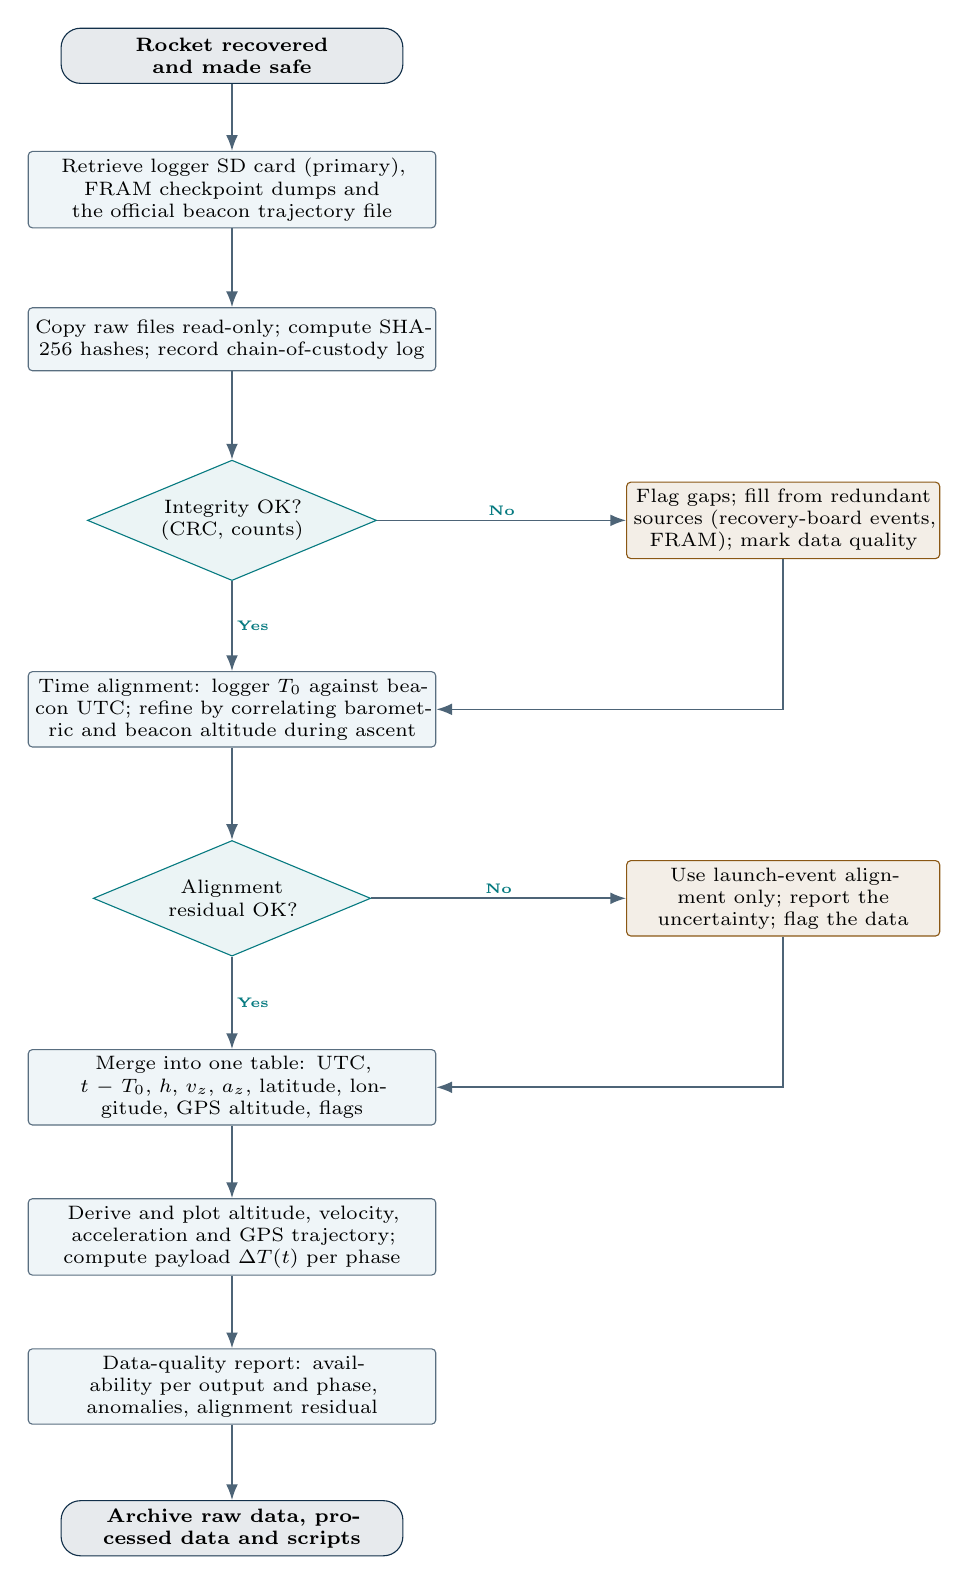
\begin{tikzpicture}
\node[term] (p1) at (0,0) {Rocket recovered and made safe};
\node[proc] (p2) at (0,-1.7) {Retrieve logger SD card (primary), FRAM checkpoint dumps and the official beacon trajectory file};
\node[proc] (p3) at (0,-3.6) {Copy raw files read-only; compute SHA-256 hashes; record chain-of-custody log};
\node[dec] (d1) at (0,-5.9) {Integrity OK?\\(CRC, counts)};
\node[fault,text width=3.8cm] (f1) at (7.0,-5.9) {Flag gaps; fill from redundant sources (recovery-board events, FRAM); mark data quality};
\node[proc] (p4) at (0,-8.3) {Time alignment: logger $T_0$ against beacon UTC; refine by correlating barometric and beacon altitude during ascent};
\node[dec] (d2) at (0,-10.7) {Alignment\\residual OK?};
\node[fault,text width=3.8cm] (f2) at (7.0,-10.7) {Use launch-event alignment only; report the uncertainty; flag the data};
\node[proc] (p5) at (0,-13.1) {Merge into one table: UTC, $t-T_0$, $h$, $v_z$, $a_z$, latitude, longitude, GPS altitude, flags};
\node[proc] (p6) at (0,-15.0) {Derive and plot altitude, velocity, acceleration and GPS trajectory; compute payload $\Delta T(t)$ per phase};
\node[proc] (p7) at (0,-16.9) {Data-quality report: availability per output and phase, anomalies, alignment residual};
\node[term] (p8) at (0,-18.7) {Archive raw data, processed data and scripts};
\draw[flow] (p1) -- (p2);
\draw[flow] (p2) -- (p3);
\draw[flow] (p3) -- (d1);
\draw[flow] (d1.south) -- node[lab,right]{Yes} (p4.north);
\draw[flow] (d1.east) -- node[lab,above]{No} (f1.west);
\draw[flow] (f1.south) |- (p4.east);
\draw[flow] (p4) -- (d2);
\draw[flow] (d2.south) -- node[lab,right]{Yes} (p5.north);
\draw[flow] (d2.east) -- node[lab,above]{No} (f2.west);
\draw[flow] (f2.south) |- (p5.east);
\draw[flow] (p5) -- (p6);
\draw[flow] (p6) -- (p7);
\draw[flow] (p7) -- (p8);
\end{tikzpicture}
\caption{Post-flight data pipeline that turns the logger files and the organiser beacon track into one evidence package covering all four required outputs.}
\label{fig:dataflow}
\end{figure}

%======================================================================
\section{Verification plan}
%======================================================================
Methods follow the usual inspection, analysis, demonstration and test categories \cite{nasase}; MDR needs the plan, not the results \cite{rtc2027app07}.

\small
\rowcolors{2}{Pale}{white}
\begin{longtable}{@{}L{11mm}L{23mm}L{70mm}L{42mm}@{}}
\toprule\rowcolor{VeryLight}\textbf{ID}&\textbf{Method}&\textbf{Planned evidence}&\textbf{Initial pass criterion (team target)}\\\midrule\endfirsthead
\toprule\rowcolor{VeryLight}\textbf{ID}&\textbf{Method}&\textbf{Planned evidence (continued)}&\textbf{Pass criterion}\\\midrule\endhead
\bottomrule\endlastfoot
V-01 & Test & Replay recorded and simulated histories through the A and B logic with injected noise and spikes. & No false apogee/main trigger in $\ge1000$ randomised replays; confirm both sensor inputs on A/B.\\
V-02 & Test & Logger timing: loop jitter, buffer occupancy, SD latency, forced SD errors. & Jitter $<10\%$ of the 5\,ms period; no overruns; buffer $<50\%$ full.\\
V-03 & Demonstration & Force a core stall mid-sequence; confirm watchdog restart and state restore from scratch registers. & State correct; log gap $\le3$\,s.\\
V-04 & Test & Interrupt supply for 1\,ms, 20\,ms, 100\,ms and 1\,s in every flight state on logger and recovery boards. & Correct state restored from FRAM; outputs stay low throughout; POWER\_LOSS flagged.\\
V-05 & Demonstration & Fault injection with safe test loads: A disabled, B disabled, both enabled. & Each channel alone releases drogue then main in 10 of 10 trials.\\
V-06 & Test & Power endurance with realistic logging; connector pull and vibration retention. & Runs $\ge1.5$\,h with $\ge25\%$ capacity margin.\\
V-07 & Analysis & Acceleration envelope against thrust curve, mass and deployment shock (Sec.~\ref{sec:accel}). & ADXL375 baseline range verified against $k\,a_{pk}$ and MPU6050 range recorded.\\
V-08 & Test & Thermal probes: common-bath offset calibration, step response, 1\,h data-completeness run. & $\Delta T$ uncertainty $\le0.3\,^{\circ}$C; completeness $\ge99\%$.\\
V-09 & Test & Barometer ports: pressure chamber or vented-bay test with representative pressure profile. & A and B altitude agree within $\pm5$\,m.\\
V-10 & Demonstration & Dry run of the post-flight pipeline (Fig.~\ref{fig:dataflow}) on a ground or simulated data set. & All four outputs produced; alignment residual $\le1$\,s.\\
V-11 & Inspection & Wiring, labels, strain relief, arming-switch access and polarity \cite{rtc2027app03}. & No findings.\\
V-12 & Analysis & Mass, power and cost budget and FMEA update for PDR \cite{rtc2027app12}. & Budget and FMEA approved by lead.\\
V-13 & Test & Unpowered/inert ingress and pressure-vent compatibility; media retrieval after splash. & No wet primary storage; acceptable barometric response, test limits TBD.\\
V-14 & Demonstration & Official GPS beacon mounted in representative bay: position reception, status, battery and trajectory export. & Position packets received; documented export method.\\
V-15 & Inspection/test & Protected cells, individual fuses, polarity, mounting, peak load and 1.5-hour endurance. & No unsafe heating or disconnection; measured endurance meets rule.\\
V-16 & Test & Representative switching/noise transients with safe inert loads and mixed sensor activity. & No unintended output or unreported critical reset.\\
V-17 & Demonstration & Configuration checksum, arming procedure and independent two-person read-back. & Correct configuration and safe state confirmed.\\
\end{longtable}
\normalsize

%======================================================================

% ======================================================================
\section{Preliminary scored electronics FMEA}
\label{sec:fmea}
% ======================================================================
This is the MDR-level \emph{initial} risk register, following the organiser's FMEA example \cite{rtc2027app12}. Ratings are team assumptions, not measured reliabilities: Severity (S), Occurrence (O) and Detectability (D) range from 1 (low) to 5 (high or difficult to detect); risk priority is $RPN=S\times O\times D$. High-severity hazards still receive priority even when their RPN is low. Final criteria and residual risk acceptance belong to the team safety/recovery leads.

\footnotesize
\rowcolors{2}{Pale}{white}
\begin{longtable}{@{}L{9mm}L{30mm}L{32mm}c c c r L{37mm}@{}}
\toprule\rowcolor{VeryLight}\textbf{ID}&\textbf{Failure mode}&\textbf{Effect}&\textbf{S}&\textbf{O}&\textbf{D}&\textbf{RPN}&\textbf{Mitigation / owner}\\\midrule\endfirsthead
\toprule\rowcolor{VeryLight}\textbf{ID}&\textbf{Failure mode}&\textbf{Effect}&S&O&D&RPN&\textbf{Mitigation / owner}\\\midrule\endhead
\bottomrule\endlastfoot
F01 & Common-mode recovery software defect & Both stages delayed or fail & 5 & 3 & 4 & 60 & Diverse channel B, review, replay tests; Recovery lead\\
F02 & Release mechanism jams & Chute not deployed & 5 & 3 & 4 & 60 & Independent initiation; mechanical load tests; Recovery + structures\\
F03 & Static-port blockage or transient & Wrong altitude/recovery event & 5 & 3 & 3 & 45 & Port separation, plausibility, chamber test; Recovery\\
F04 & Recovery cell/connector fails & One recovery channel lost & 5 & 2 & 3 & 30 & Separate cells and wiring; endurance + vibration; Electronics\\
F05 & Spurious arming/output & Premature release or hazardous event & 5 & 2 & 3 & 30 & Physical arming, default low outputs, continuity checks; Recovery\\
F06 & MCU reset/brownout & Data lost or recovery state uncertain & 4 & 3 & 3 & 36 & FRAM checkpoint, reset discrimination, fault injection; Avionics\\
F07 & IMU saturation & Missing acceleration peaks & 3 & 4 & 2 & 24 & Simulated envelope and optional high-g sensor; Avionics\\
F08 & SD-card write failure & Lost flight/payload evidence & 3 & 3 & 2 & 18 & Buffering, CRC, sync and recovery test; Logger lead\\
F09 & GPS beacon/radio failure & Rocket location unavailable & 4 & 3 & 3 & 36 & Independent beacon test, antenna placement, range check; GPS lead\\
F10 & Thermal probes detach/drift & Invalid payload result & 2 & 3 & 2 & 12 & Probe retention and calibration; Payload lead\\
F11 & Wiring/PCB mount loosens & Intermittent signals or loss of power & 4 & 3 & 3 & 36 & Labelled locking connectors, strain relief; Integration\\
F12 & Water ingress at splashdown & Lost primary data or damaged beacon & 4 & 4 & 3 & 48 & Sealed bay, pressure-vent separation, ingress test V-13; Integration\\
F13 & Li-ion short, overheating, cell abuse & Fire/thermal or electrical hazard & 5 & 2 & 4 & 40 & Protected/secured cells, fuse and handling V-15; Safety\\
F14 & EMI / transient coupling & False sensor reading, reset or output & 5 & 2 & 3 & 30 & Segregation, grounding/EMI review and V-16; Electronics\\
F15 & Wrong configuration or arming order & Unsafe or missed recovery event & 5 & 3 & 4 & 60 & Two-person checklist, config checksum, V-17; Recovery\\
\end{longtable}
\normalsize

\textbf{Risk-closure expectations:} Document the recovery-lead decision on F01--F05 before design freeze; update S/O/D after preliminary testing; and attach V-01 to V-12 test identifiers to the final FMEA worksheet. All named owners are \emph{roles}, not confirmed individual assignments.

% ======================================================================
\section{Development roadmap, responsibility allocation and MDR slide handover}
\label{sec:schedule}

\subsection{Near-term MDR Gantt chart and dependencies}
\begin{figure}[htbp]\centering
\resizebox{\linewidth}{!}{%
\begin{ganttchart}[time slot format=isodate,time slot unit=day,
  vgrid,hgrid,bar height=.55,
  x unit=0.88cm,y unit chart=.57cm,
  title label font=\scriptsize,bar label font=\scriptsize,
  bar/.append style={fill=Teal!70,draw=Teal!90!black},
  milestone/.append style={fill=Amber,draw=Amber}]{2026-11-04}{2026-11-13}
\gantttitlecalendar{month=shortname,day}\\
\ganttbar{Requirements / mission targets}{2026-11-04}{2026-11-05}\\
\ganttbar{Recovery and GPS interfaces}{2026-11-05}{2026-11-07}\\
\ganttbar{BOM, procurement, mass}{2026-11-06}{2026-11-08}\\
\ganttbar{Simulation / profile inputs}{2026-11-07}{2026-11-09}\\
\ganttbar{FMEA and verification}{2026-11-08}{2026-11-10}\\
\ganttbar{Extract and integrate MDR slides}{2026-11-10}{2026-11-11}\\
\ganttbar{Internal review}{2026-11-12}{2026-11-12}\\
\ganttmilestone{Single team MDR submission}{2026-11-13}
\end{ganttchart}}
\caption{Team planning Gantt chart (proposal, not actual completed work). Dependencies: requirements before interface freeze; flight-dynamics simulation before numeric sensor thresholds; equipment and payload agreement before BOM freeze; risks/verification before final slide review. Responsibility assignment remains pending.}
\label{fig:gantt}
\end{figure}
\textbf{Dependency flow:} Define objectives $\rightarrow$ derive requirements $\rightarrow$ constrain sensors and recovery interface $\rightarrow$ update BOM/mass/power $\rightarrow$ evaluate FMEA and verification $\rightarrow$ merge with flight simulation $\rightarrow$ review and submit. Follow-up PDR/CDR schedule remains indicative until organiser dates and team owners are confirmed.

% ======================================================================
The following dates use the stated MDR closing date of \textbf{13 November 2026}; they are an internal \emph{proposal}. The team leader must assign named members before submission. Later PDR/CDR month references are planning windows, not exact confirmed organiser dates \cite{rtc2027app01,rtc2027app07}.

\small
\rowcolors{2}{Pale}{white}
\begin{longtable}{@{}L{27mm}L{63mm}L{38mm}L{23mm}@{}}
\toprule\rowcolor{VeryLight}\textbf{Target}&\textbf{Task / deliverable}&\textbf{Responsible role}&\textbf{Stage}\\\midrule\endfirsthead
\toprule\rowcolor{VeryLight}\textbf{Target}&\textbf{Task}&\textbf{Role}&\textbf{Stage}\\\midrule\endhead
\bottomrule\endlastfoot
4--5 Nov 2026 & Freeze initial AV/RC/PW/GPS/PL requirements and thermal mission criteria & Avionics + payload leads (assign names) & MDR\\
5--7 Nov 2026 & Confirm three-power-domain interfaces and preliminary recovery-release concept & Recovery + integration leads & MDR\\
6--8 Nov 2026 & Compile supplier-link BOM, cost estimates and mass/power allocations & Procurement + electrical leads & MDR\\
7--9 Nov 2026 & Insert rocket flight-simulation bounds (replace Fig.~\ref{fig:missionprofile}), or flag missing inputs and decision gate & Flight dynamics + avionics & MDR\\
8--10 Nov 2026 & Complete numbered verification plan and initial FMEA; risk review & Safety + avionics leads & MDR\\
10--11 Nov 2026 & Extract two/three concise slides into the master MDR & MDR editor + electronics leads & MDR\\
12 Nov 2026 & Internal design review, source audit and final PDF export & Team leader + reviewers & MDR\\
13 Nov 2026 & Submit the \emph{single team} searchable MDR PDF & Team leader & MDR\\
After MDR (dates TBD) & Prototype logger + both recovery paths; review components against simulation & Avionics + recovery & PDR\\
Before CDR (dates TBD) & Integrated bench, actuation, fault injection, endurance and environmental tests; revise verification matrix & All electronics teams & CDR\\
Flight readiness (TBD) & Demonstrate safe arming, GPS reporting and launch checklist compliance & Recovery + GPS + team lead & FRR\\
\end{longtable}
\normalsize

\subsection*{Proposed MDR integration map (electronics contribution)}
\small
\begin{tabularx}{\linewidth}{@{}L{22mm}Y L{40mm}@{}}
\toprule\rowcolor{VeryLight}\textbf{Template location}&\textbf{Material to extract}&\textbf{Responsible editor}\\\midrule
Slide 2 & Avionics, recovery and payload objectives and measurable success criteria & Team lead / payload\\
Slides 3--5 & Named responsibilities and electronics milestones/Gantt & Team lead\\
Slides 6--7 & Hardware choices, Shopee-linked costed BOM, contingency and power/mass assumptions & Procurement + avionics\\
Slide 8 & Annotated avionics-bay/recovery/GPS/payload placement with mass interfaces & Integration + structures\\
Slide 9 & Numbered functional requirements plus one simplified architecture figure & Avionics lead\\
Slide 10 & Expected flight event sequence and recovery/payload timing (link simulation) & Flight dynamics + avionics\\
Slide 11 & Development dependencies, verification plan and integration stages & Avionics + recovery\\
Slide 12 & Initial high-priority FMEA and risk reduction plan & Safety + recovery\\
\bottomrule
\end{tabularx}
\normalsize

For the \emph{final MDR}, condense this engineering annex into the team's master presentation rather than submitting all detailed flowcharts and tables independently. The design remains provisional where the mechanism, rocket simulation, complete GPS arrangement or confirmed pricing is unavailable.

\section{Decisions needed from the team}
%======================================================================
\begin{enumerate}
\item Select the release-interface arrangement (R1--R4) with the recovery lead, and approve the diverse channel B (MS5611, independent IMU, separate firmware, time back-up).
\item Provide the Pioneer-10K thrust curve, mass history and flight simulation so that $a_{pk}$ and the ADXL375 range validation (Sec.~\ref{sec:accel}) can be made, and so that $a_L$, $t_{lock}$, $v_{max}$ and $T_{apo,max}$ can be fixed.
\item Approve the FRAM checkpoint and agree the recovery-board fallback rule when no valid checkpoint exists.
\item Approve the thermal research question and success criteria, or replace them with an agreed payload using the same format.
\item Obtain quotes for release hardware, baseline ADXL375 module and the GPS beacon, and confirm how the beacon track file is retrieved.
\item Confirm bay dimensions, mounting, battery protection and measured current before procurement.
\end{enumerate}

\printbibliography[title={References}]
\end{document}